\documentclass[12pt,a4paper]{book}
\usepackage[utf8]{inputenc}                                             % Codificación
\usepackage[spanish,es-tabla]{babel}                                    % Lenguaje español, Tabla n: 
\usepackage[T1]{fontenc}                                                % Agregar fuentes con acentos
\usepackage{amsmath}                                                    % Paquetes necesarios  para matemáticas
\usepackage{amsfonts}
\usepackage{amssymb}
\usepackage{makeidx}                                                    % Paquete para indices
\usepackage{graphicx}                                                   % Para manejar imagenes
\graphicspath{{imagenes/}}                                              % Ruta de las imagenes, solo escribir nombre de la imagen
\usepackage[top=1in, left=0.9in, right=1.25in, bottom=1in]{geometry}	% Margenes
\author{Ciro Fabian Bermudez Marquez}
\title{Tesis}
\date{}
%-------------------------------------------------------------------------------
%                            Paquetes adicionales                              %
%-------------------------------------------------------------------------------
%-------------------------------------------------------------------------------
%                                Paquetes extras                               %
%-------------------------------------------------------------------------------
\setcounter{secnumdepth}{3}
\setcounter{tocdepth}{3} 
\usepackage{amsthm}
\theoremstyle{definition}
\newtheorem{axiom}{Axioma} %[chapter]
\renewcommand\theaxiom{\Roman{axiom}}

\theoremstyle{definition}
\newtheorem{property}{Propiedad} %[chapter]

\theoremstyle{definition}
\newtheorem{corollary}{Corolario} %[chapter]

\theoremstyle{definition}
\newtheorem{theorem}{Teorema} %[chapter]

\usepackage{lipsum}												% Texto de ejemplo \lipsum[1-30]
\decimalpoint													% Punto decimal en lugar de coma
\spanishsignitems												% Viñetas en lugar de cuadros
\raggedbottom													% Eliminar molestos warnings

\usepackage{comment}											% Comentarios largos
\usepackage{pdfpages}											% Incluir portada echa en Inkscape
\usepackage{setspace}											% Interlineado
\usepackage{makecell}											% Para tablas
\usepackage{xcolor}												% Colores en tablas
\usepackage{colortbl}
\usepackage{multirow}
\usepackage{array}												% Necesario para algunas tablas
\usepackage[inline]{enumitem}									% Personalizar itemize
\usepackage{multicol}											% Item 2 columns

\definecolor{Red}{RGB}{255,191,191}								% Colores definidos por el usuario

\usepackage[nottoc]{tocbibind}									% Bibliografia en table of contents

\usepackage[figuresright]{rotating}								% Rotar figuras con caption
\usepackage{subcaption}											% Subfiguras
%-------------------------------------------------------------------------------
%                            Comandos matematicos                              %
%-------------------------------------------------------------------------------
\usepackage{steinmetz}											% Para representar fasores
\usepackage{bm}													% Bold math  \bm command
\newcommand{\binomb}[2]{\genfrac{[}{]}{0pt}{}{#1}{#2}}
%-------------------------------------------------------------------------------
%                        Paquetes para hipervinculos                           %
%-------------------------------------------------------------------------------
\usepackage[hidelinks]{hyperref}								% Añade los bookmarks y le quita la caja roja, \url{}
\urlstyle{same}
%-------------------------------------------------------------------------------
%                           Estilos de encabezados                             %
%-------------------------------------------------------------------------------
\usepackage{fancyhdr, blindtext}								% Libreria para encabezados

\renewcommand{\chaptermark}[1]{\markboth{#1}{}}					% Capitulos y secciones en minusculas
\renewcommand{\sectionmark}[1]{\markright{#1}}

\fancypagestyle{normalstyle}{%
  \fancyhf{}													% Reinicial estilos de header y footer
	\fancyhead[LE,RO]{\thepage}
	\fancyhead[LO]{\nouppercase{\rightmark}}
	\fancyhead[RE]{\nouppercase{\leftmark}}
	\renewcommand{\headrulewidth}{0.4pt}
	\renewcommand{\footrulewidth}{0pt}
	\setlength{\headheight}{14.62pt}
}

\fancypagestyle{Resumen}{%
  \fancyhf{}													% Reinicial estilos de header y footer
	\fancyhead[LE,RO]{\thepage}
	\fancyhead[LO]{\nouppercase{Resumen}}
	\fancyhead[RE]{\nouppercase{Resumen}}
	\renewcommand{\headrulewidth}{0.4pt}
	\renewcommand{\footrulewidth}{0pt}
	\setlength{\headheight}{14.62pt}
}
%-------------------------------------------------------------------------------
%                            Libreria de codigos                               %
%-------------------------------------------------------------------------------
% Paquetes necesarios
\usepackage{listings}
\usepackage{xcolor}

% Colores para tablas
\definecolor{Gray}{RGB}{230,230,230}
\definecolor{Red}{RGB}{255,191,191}

% Colores personalizados
\definecolor{verde}{rgb}{0,0.6,0}
\definecolor{gris}{RGB}{253, 253, 253}
\definecolor{grisfuerte}{RGB}{140, 140, 140}

% Deficion de lenguajes perzonalizados

% Estilos MATLAB
\lstdefinestyle{MATLAB}{
	language=MATLAB,
	basicstyle=\linespread{1}\tiny\fontfamily{pcr}\selectfont,
	backgroundcolor=\color{gris},
	frame=single,
	frameround=tttt,
	rulecolor=\color{black},
	commentstyle=\color{verde},
	keywordstyle=\color{blue}, %magenta
	stringstyle=\color{grisfuerte},                  
	captionpos=t,                    
	breaklines=true,                       
	breakatwhitespace=false,
	showspaces=false,                
	showstringspaces=false,
	showtabs=false,
	keepspaces=true,
	columns=flexible,
	tabsize=4,   
}

\lstdefinestyle{VHDL}{
	language=VHDL,
	basicstyle=\linespread{1}\tiny\fontfamily{pcr}\selectfont,
	backgroundcolor=\color{gris},
	frame=single,
	frameround=tttt,
	rulecolor=\color{black},
	commentstyle=\color{verde},
	keywordstyle=\color{blue}, %magenta
	stringstyle=\color{grisfuerte},                  
	captionpos=t,                    
	breaklines=true,                       
	breakatwhitespace=false,
	showspaces=false,                
	showstringspaces=false,
	showtabs=false,
	keepspaces=true,
	columns=flexible,
	tabsize=4,
	upquote=true,
}


\lstdefinestyle{VHDL_TEXT}{
	language=VHDL,
	basicstyle=\linespread{1}\footnotesize\fontfamily{pcr}\selectfont,
	backgroundcolor=\color{gris},
	frame=single,
	frameround=tttt,
	rulecolor=\color{black},
	commentstyle=\color{verde},
	keywordstyle=\color{blue}, %magenta
	stringstyle=\color{grisfuerte},                  
	captionpos=t,                    
	breaklines=true,                       
	breakatwhitespace=false,
	showspaces=false,                
	showstringspaces=false,
	showtabs=false,
	keepspaces=true,
	columns=flexible,
	tabsize=4,
	upquote=true,
}


\lstdefinestyle{C}{
	language=C,
	basicstyle=\linespread{1}\tiny\fontfamily{pcr}\selectfont,
	backgroundcolor=\color{gris},
	frame=single,
	frameround=tttt,
	rulecolor=\color{black},
	commentstyle=\color{verde},
	keywordstyle=\color{blue}, %magenta
	stringstyle=\color{grisfuerte},                  
	captionpos=t,                    
	breaklines=true,                       
	breakatwhitespace=false,
	showspaces=false,                
	showstringspaces=false,
	showtabs=false,
	keepspaces=true,
	columns=flexible,
	tabsize=4,
	upquote=true,    
}

\renewcommand{\lstlistingname}{Código}% Listing -> Algorithm
\renewcommand{\lstlistlistingname}{Lista de códigos}% 

%-------------------------------------------------------------------------------
%                           Caption en negritas                                %
%-------------------------------------------------------------------------------
\usepackage[labelfont=bf]{caption}
\captionsetup{labelfont=bf}


%-------------------------------------------------------------------------------
%                           Lista de conceptos                                %
%-------------------------------------------------------------------------------
\usepackage[nonumberlist,nogroupskip,toc,style=super]{glossaries}
\setlength{\glsdescwidth}{0.7\textwidth}

\makeglossaries

\newglossaryentry{FPGA}
{
    name=FPGA, %% $\qquad\qquad\qquad\qquad$
    description={Field Programmable Logic Array}
}

\newglossaryentry{RNG}
{
    name=RNG,
    description={Random Number Generator}
}

\newglossaryentry{TRNG}
{
    name=TRNG,
    description={True Random Number Generator}
}

\newglossaryentry{TERO}
{
    name=TERO,
    description={Transient Effect Ring Oscillator}
}

\newglossaryentry{ERO-TRNG}
{
    name=ERO-TRNG,
    description={Elementary ring oscillator based TRNG}
}

\newglossaryentry{COSO-TRNG}
{
    name=COSO-TRNG,
    description={Coherent sampling ring oscillator based TRNG}
}

\newglossaryentry{MURO-TRNG}
{
    name=MURO-TRNG,
    description={Multi-ring oscillator based TRNG}
}


\newglossaryentry{TERO-TRNG}
{
    name=TERO-TRNG,
    description={Transient effect ring oscillator based TRNG}
}

\newglossaryentry{PLL-TRNG}
{
    name=PLL-TRNG,
    description={Phase-locked loop based TRNG}
}


\newglossaryentry{STR-TRNG}
{
    name=STR-TRNG,
    description={Self-timed ring based TRNG}
}


%-------------------------------------------------------------------------------
%                             Archivos a incluir                               %
%-------------------------------------------------------------------------------
\includeonly{
	portada,
	agradecimientos,
	resumen,
	ch1,
	ch2,
	ch3,
	ch4,
	ch5,
	ch6,
    test,
	Ap_A
}
%-------------------------------------------------------------------------------
%-------------------------------------------------------------------------------
\begin{document}
	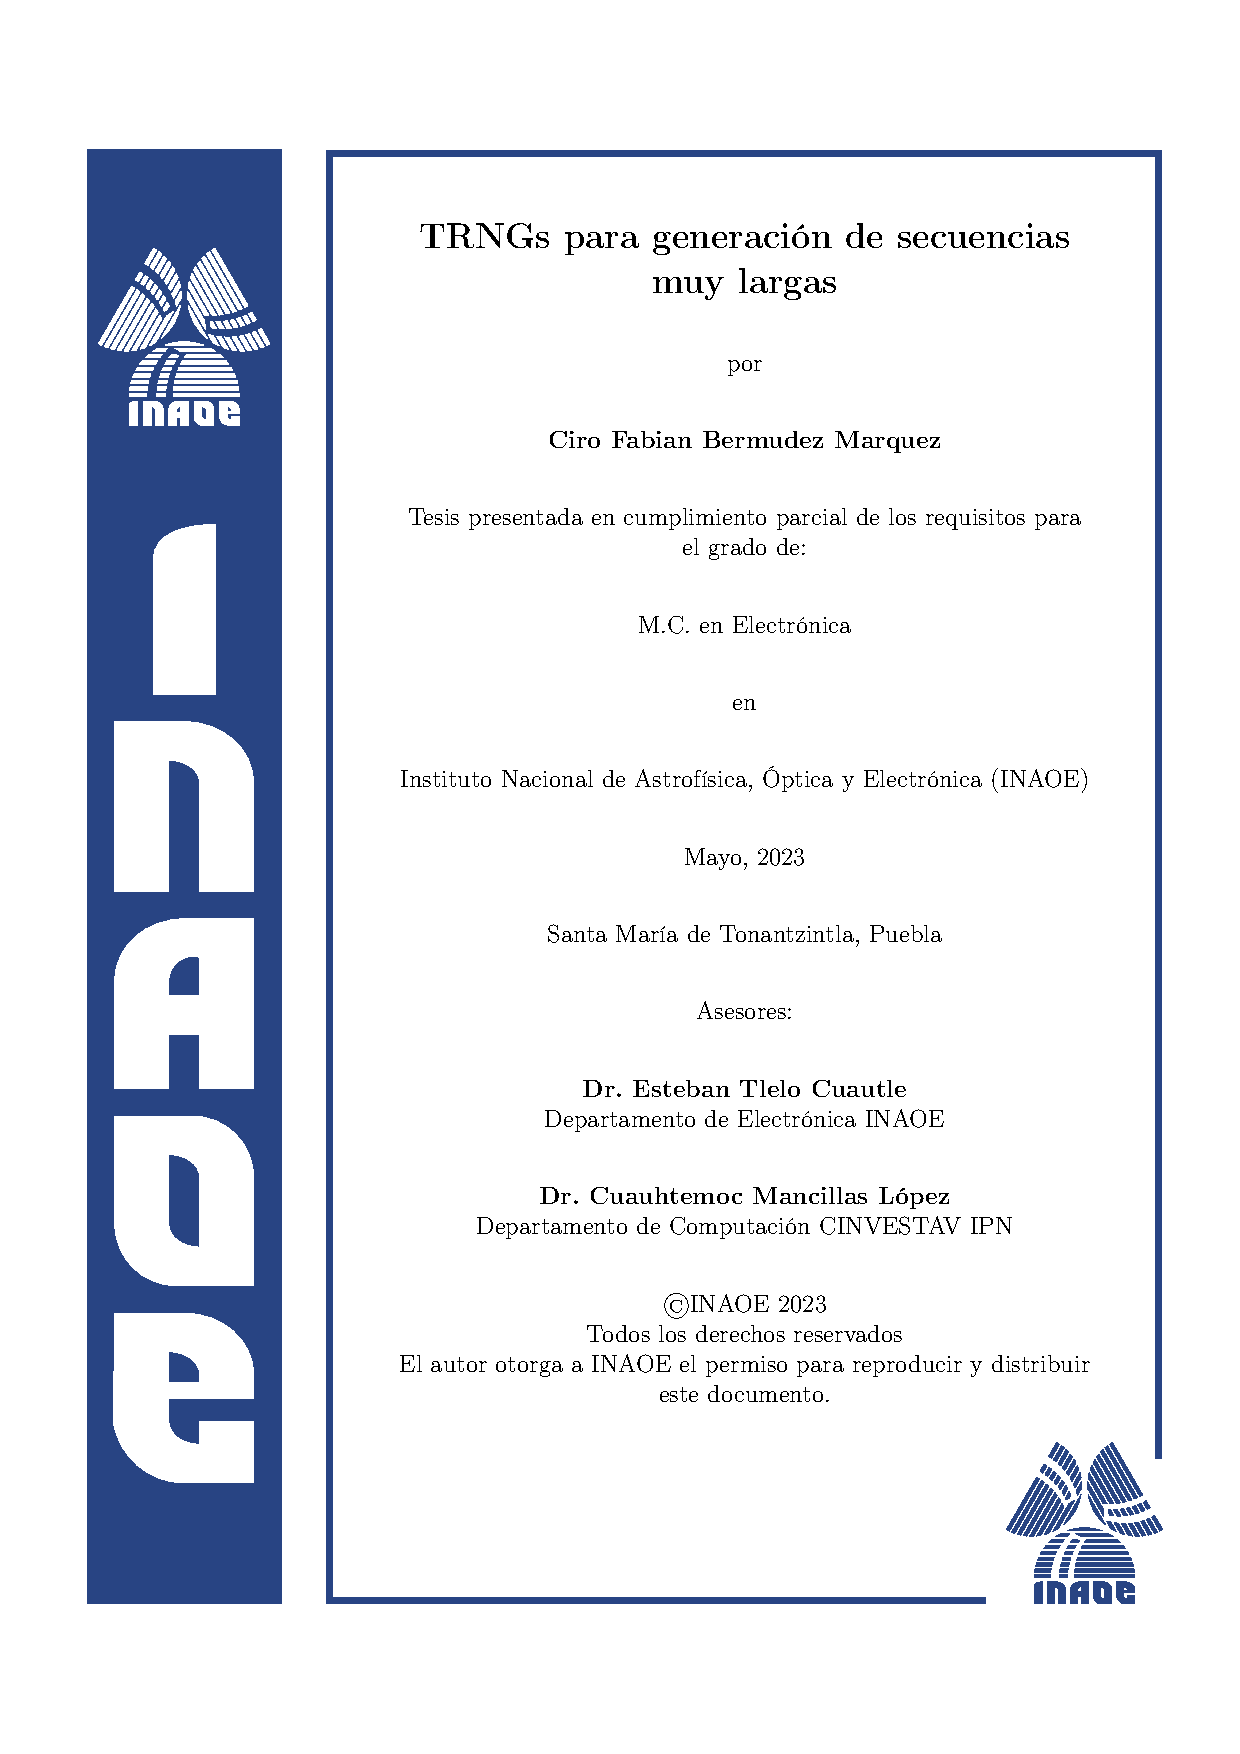
\includepdf[pages=-]{portada/main.pdf}

	\thispagestyle{empty}								            % Limpiar estilos de pagina

\frontmatter
\onehalfspacing										                % Desde este punto interlineado de 1.5
% 	\spacing{1.213}
	\chapter{Agradecimientos}
    
    \begin{itemize}
        \item Para mi familia, mis hermanos Efraín, Alejandro y mis padres Juana y Efrain, les agradezco con todo mi corazón.
        \item A mis compañeros de laboratorios, Victor, Juan, Julio gracias por ayudarme a resolver mis dudas.
        \item A mi novia Julisa.
        \item A mi asesor Esteban por su infinita paciencia y apoyo.
    \end{itemize}



\pagestyle{normalstyle}									            % Estilos de pagina personalizados
\tableofcontents            								        % Genera el índice
\addcontentsline{toc}{chapter}{\contentsname}

\listoffigures              								        % Indice de figuras
\listoftables               								        % Indice de tablas

\lstlistoflistings                                                  % Indice de códigos
\addcontentsline{toc}{chapter}{\lstlistlistingname}


\printglossary[title=Lista de abreviaciones, toctitle=Lista de abreviaciones] % Glosario

	\chapter{Resumen}
    
    En esta tesis se diseño e implementó un TRNG híbrido en la FPGA Xilinx Artix 7 xc7a35tcpg236-1 sobre la tarjeta de desarrollo Digilent Basys 3. Se utilizó un núcleo ERO-TRNG para generar una semilla de 64 bits que funciona como condición inicial para un mapa caótico bidimensional. Haciendo uso de la operación mod 256 se extraen 16 bits aleatorios por cada iteración del mapa. 

    En este trabajo se presenta toda la teoría necesaria para comprender los generadores de números aleatorios así como su clasificación, fuentes de aleatoriedad, parámetros de evaluación pruebas estadísticas y arquitecturas de núcleos TRNG específicas para FPGA. Se estudian brevemente las características principales de los mapas caóticos como puntos fijos, estabilidad lineal, diagramas de bifurcación y diagramas de cobwebs. Después se expone la metodología de diseño para implementar en FPGA el mapa caótico bidimensional y el núcleo ERO-TRNG utilizando el lenguaje de descripción de hardware VHDL. El mapa caótico se implementó utilizando aritmética de punto fijo de 64 bits, 3 bits para la parte entera, 60 bits para la fraccionaria y un bit de signo y para comprobar su funcionamiento se empleó un simulador desarrollado lenguaje C. Posteriormente se analizó el dominio de atracción del mapa para diferentes parámetros con el fin de poder seleccionar un rango en que las condiciones iniciales produzcan caos, por ultimó se utilizaron multiplicadores de una sola constante para reducir el uso de recursos. Utilizando diversos elementos digitales básicos y el núcleo ERO-TRNG se diseño un generador de semillas de 64 bits que alimenta a las condiciones iniciales del mapa caótico. Finalmente las secuencias binarias obtenidas por el TRNG híbrido se mandaron a una computadora utilizando el protocolo de comunicación RS232 y se analizaron con las pruebas estadísticas NIST SP 800-22.

	\pagestyle{Resumen}	
	
\mainmatter
\pagestyle{normalstyle}	
	\chapter{Introducción}
	
	\section{Objetivos}
	
		\subsection{Objetivo general}
			\begin{itemize}
				\item Diseño e implementación en FPGA de un TRNG híbrido para la generación de secuencias muy largas y utilizarla para cifrar una imagen.
			\end{itemize}
		
		\subsection{Objetivos específicos}
			\begin{enumerate}
                \item Investigar el estado del arte de diferentes generadores de números aleatorios y sus aplicaciones en cifradores.
                \item Estudiar los diferentes tipos de generadores de números aleatorios y analizar sus características principales.
                \item Estudiar la teoría de los mapas caóticos y su utilidad en generadores de números aleatorios.
                \item Diseñar un generador de números aleatorios hibrido 
			\end{enumerate}


	\chapter{Random Number Generators (RNGs)}

    En este capitulo se presentan los conceptos necesarios para comprender cómo funcionan las diferentes clases de generadores de números aleatorios, sus fuentes de aleatoriedad, sus principales características, AGREGAR MÄS DESPUES. 

    \section{Clasificación de los RNGs}

        Dado el amplio rango de aplicaciones de los RNG, existan diferentes clases de RNG que satisfacen diversas necesidades. Basándonos en el método utilizado para generar números aleatorios, podemos distinguir dos tipos fundamentales de RNG:
	        
        \begin{enumerate}
            \item Generadores de números aleatorios deterministas (DRNG/PRNG)
            
                También conocidos como generadores de números pseudo-aleatorios o Pseudo-Random Numger Generators (PRNG), son sistemas que producen una secuencia de aspecto aleatorio de forma matemática, es decir, hay un algoritmo subyacente y debido a esto los Deterministic Random Number Generators (DRNG) son fáciles de implementar en dispositivos lógicos. Si se conoce el algoritmo, la salida del generador es predecible. Incluso cuando no se conoce el algoritmo pero se han guardado algunas de las secuencias de salida del generador, su comportamiento durante la secuencia guardada puede utilizarse en futuros ataques. Los números producidos parecen aleatorios a corto plazo, pero la secuencia es periódica, normalmente con un periodo largo. Para producir una salida menos predecible, estos generadores utilizan valores de inicialización llamados semillas para empezar a generar números \cite{Nist2010}. Para cada semilla se genera una secuencia diferente. Por esta razón, los DRNG deben ser computacionalmente seguros, el algoritmo no debe poder adivinarse computacionalmente y su valor inicial nunca debe reutilizarse. La reutilización del valor inicial puede evitarse guardando el último valor haciendo uso de un contador y utilizando el siguiente valor del contador la próxima vez. La secuencia de salida de un buen DRNG está perfectamente distribuida de manera uniforme, en otras palabras, tienen buenas propiedades estadísticas. Además, los DRNGs consiguen altas tasas de bits de salida y suelen utilizarse como generadores de claves en los cifrados de flujo \cite{Badrignans2011}.
            
            \item Generadores de números aleatorios verdaderos (TRNG)
            
                Los True Random Number Generators (TRNG) son sistemas que extraen la aleatoriedad de fenómenos aleatorios no algorítmicos impredecibles como fluctuaciones de temperatura, decaimiento radiactivo, ruido de radio ambiental, tiempos de acceso al disco duro o interacciones del usuario con el PC, jitter, entre otros. A diferencia de los DRNG, que utilizan fórmulas matemáticas para generar números aleatorios, los TRNG producen datos aleatorios reales que no se pueden predecir. Sin embargo, debido a que los procesos físicos utilizados por los TRNG están sujetos a fluctuaciones, la calidad de la secuencia aleatoria generada puede presentar algunos defectos estadísticos, como el sesgo.
                
                Dado que los procesos físicos están sujetos a fluctuaciones, las características estadísticas de los TRNG suelen ser peores que las de los DRNG y están estrechamente relacionadas con la calidad de la fuente de entropía y con el método de extracción de la aleatoriedad. La velocidad final de los TRNG está limitada por el espectro de la señal aleatoria y por el principio utilizado para extraer la entropía de la misma, por ejemplo, la frecuencia de muestreo vinculada al espectro del ruido. En general, los TRNG son, más lentos que los DRNG. Dependiendo de la fuente utilizada los TRNG se pueden dividir en:
            
            \begin{itemize}
                \item Físicos (PTRNG), utilizan ruido físico a nivel de electrones presente en todos los semiconductores. Es un dispositivo físico y utiliza ruido físico.
                \item No físicos (NPTRNG), puede no ser dispositivos físicos, sino más bien una pieza de software que utilizan fuentes de aleatoriedad no físicas, como las interacciones del usuario con un sistema operativo, por mencionar algunas el movimiento del cursor del mouse.
            \end{itemize}
        \end{enumerate}
	
        La imprevisibilidad de los generadores de números aleatorios deterministas está garantizada computacionalmente, mientras que la imprevisibilidad de los generadores verdaderamente aleatorios está garantizada por fenómenos físicos aleatorios y se caracteriza por la tasa de entropía a la salida del generador. Tanto los TRNG como los DRNG tienen sus ventajas y desventajas, por lo que muchos sistemas criptográficos utilizan RNG híbridos. Los generadores de números aleatorios híbridos, conocidos como Hybrid Random Number Generators (HRNG) combinan las fortalezas de los DRNG (rápidos y de buena calidad) sembrados repetidamente por un TRNG (lento pero impredecible). Es importante encontrar un equilibrio entre la velocidad del generador y su imprevisibilidad ajustando el intervalo de tiempo entre semillas y el tamaño de la semilla. En función de su implementación, existen dos tipos de RNG híbridos:
	
        \begin{enumerate}		
            \item Generadores de números aleatorios verdaderos híbridos
            
            Combinan un TRNG con un postprocesamiento criptográfico. El postprocesamiento criptográfico asegura el secreto hacia adelante y hacia atrás de los números aleatorios producidos, no pueden calcularse los valores pasados o los futuros a partir del valor actual. Si la fuente física falla, también garantiza unas propiedades estadísticas perfectas de los datos de salida, ya que el núcleo de un postprocesamiento criptográfico suele ser un cifrador. La tasa de bits de salida de un TRNG híbrido está limitada por la del núcleo del TRNG.
            
            \item Generadores de números aleatorios deterministas híbridos. 
            
                Utilizan un TRNG para generar periódicamente semillas para un DRNG. Dado que la salida de un DRNG es predecible si conocemos su semilla, ir renovando la semilla mediante un TRNG puede reducir la predictibilidad de un DRNG híbrido. Además la secuencia de salida de un generador de este tipo es perfectamente uniforme, lo que podría no ser el caso de un TRNG puro. Su tasa de bits de salida viene determinada por la tasa de bits del DRNG subyacente, ya que se pueden producir números aleatorios mientras no se alcance el periodo de repetición del DRNG.
        \end{enumerate}

        Para garantizar la seguridad de las claves confidenciales, es fundamental que se generen dentro del sistema criptográfico. Dado que la mayoría de los sistemas criptográficos actuales se implementan en dispositivos lógicos y sistemas digitales utilizando algoritmos y protocolos criptográficos, es natural que la investigación se centre en la implementación de generadores de números aleatorios en dispositivos lógicos, como los Field-Programmable Gate Arrays (FPGA). Esto ayuda a prevenir el acceso no autorizado a las claves y garantiza que sean generadas de manera segura y confiable dentro del sistema criptográfico.
    
        A pesar de la menor velocidad de los TRNG, estos se utilizan con más frecuencia en aplicaciones criptográficas que los DRNG. Los TRNG son las únicas primitivas criptográficas que no han sido objeto de normalización hasta ahora. Sin embargo, antes de utilizar un generador en la práctica, el principio de funcionamiento y su implementación dentro de un módulo criptográfico deben ser validados por una institución acreditada como parte de un proceso de evaluación de seguridad. Los generadores que no tienen un certificado de seguridad se consideran inseguros en cuanto a su uso en aplicaciones criptográficas. Por este motivo, es de gran interés el estudio de los principales TRNG existentes y sus características.

	\section{Estructura de los TRNG}	

        La estructura general de un TRNG se muestra en la Figura \ref{fig:A1_TRNG_estructura}. El generador debe utilizar un proceso físico incontrolable como fuente de aleatoriedad. Dado que los fenómenos físicos utilizados en los TRNG son en su mayoría procesos analógicos, suele ser necesario algún método que permita la conversión de datos del dominio analógico al digital. Se puede incluir una conversión de analógico a digital en el procedimiento de extracción de aleatoriedad. La señal binaria sin procesar obtenida, el llamado ruido digital, puede tener baja entropía, malas propiedades estadísticas o ambas. En este caso, se pueden usar algunos algoritmos de postprocesamiento para mejorar los parámetros estadísticos del flujo de bits de salida. Sin embargo, el postprocesamiento de la salida del TRNG a veces puede enmascarar una falla grave en el generador. Las pruebas estadísticas estándar pueden entonces fallar en detectar la debilidad enmascarada. Por lo tanto, se recomienda tener la posibilidad de probar el ruido digital sin procesar o Raw Bit Signal (RBS). La seguridad del generador se puede aumentar si las pruebas estadísticas se aplican sobre la marcha y si están diseñadas para adaptarse al principio de funcionamiento del generador teniendo presente sus posibles debilidades. \cite{Badrignans2011}
			
        \begin{figure}[hbtp]
            \caption{Estructura general de un TRNG \cite{Badrignans2011}.}
            \centering
            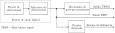
\includegraphics[width=0.9\textwidth]{A0_TRNG_estructura}
            \label{fig:A1_TRNG_estructura}
        \end{figure}
	
        Los TRNG emplean diferentes fuentes de aleatoriedad y una gran variedad de principios para extraerla. En este sentido, resulta relevante evaluar los principales principios utilizados por los TRNG: parámetros relacionados con la calidad, parámetros relacionados con la seguridad y parámetros relacionados con el diseño.

        \begin{itemize}[noitemsep]
            \item Parámetros relacionados con la calidad
                \begin{itemize}[noitemsep]
                    \item Fuente de aleatoriedad.
                    \item Método de extracción de aleatoriedad y entropía del ruido digital.
                    \item Método de procesamiento posterior aplicado (opcional).
                    \item Tasa de bits de salida y su estabilidad.
                \end{itemize}
            \item Parámetros relacionados con la seguridad
                \begin{itemize}[noitemsep]
                    \item Existencia de un modelo matemático.
                    \item Comprobabilidad interna.
                    \item Seguridad (robustez, resistencia contra ataques).
                \end{itemize}
            \item Parámetros relacionados con el diseño
                \begin{itemize}[noitemsep]
                    \item El uso de recursos.
                    \item El consumo de energía.
                    \item Viabilidad en dispositivos lógicos y FPGAs.
                    \item Automatización del diseño.
                \end{itemize}
        \end{itemize}

        Es fundamental tener en cuenta que no todas las características de los TRNG tienen la misma relevancia en su evaluación. En particular, los parámetros relacionados con la seguridad, tales como la robustez, la disponibilidad de un modelo estocástico y la capacidad de prueba, adquieren una importancia crucial en un sistema de seguridad de datos. Su peso en la evaluación de un TRNG es significativamente mayor que el de otros parámetros, como el consumo de energía o la tasa de bits. \cite{Badrignans2011}.

    \section{Parámetros de evaluación de los TRNG}
        
        \subsection{Parámetros relacionados con la calidad}	

            \subsubsection{Fuentes de aleatoriedad en dispositivos lógicos} 

            Los TRNG pueden utilizar fuentes de ruido físicas o no físicas. Sin embardo, en el caso de los dispositivos lógicos, las fuentes de ruido físico son bastante limitadas, ya que estos dispositivos se diseñan para ser deterministas y estar en un estado bien definido en todo momento. Por lo tanto, para generar números verdaderamente aleatorios, es necesario contar con un fenómeno aleatorio incontrolable que pueda utilizarse como fuente de aleatoriedad. Los fenómenos físicos más utilizados para generar números aleatorios en los dispositivos lógicos son:
	
            \begin{itemize}[noitemsep]
                \item Señales analógicas: como el ruido de disparo de un diodo, el ruido térmico, etc.		

                \item Metaestabilidad: es la capacidad de un circuito de persistir en un estado indefinido durante un periodo de tiempo indefinido.
                
                \item Jitter del reloj: es una variación del flanco del reloj desde su posición ideal.
                
                \item Caos: es un comportamiento imprevisible de un sistema determinista, muy sensible a sus condiciones iniciales, lo que significa que incluso el más mínimo cambio en el estado inicial produce resultados muy diferentes.
            \end{itemize}		
	
            La presencia de comportamientos impredecibles en un dispositivo lógico puede tener consecuencias graves en el comportamiento del sistema global. A pesar de que estos eventos son inevitables debido a la naturaleza física de la tecnología, los vendedores de dispositivos lógicos sueles minimizarlos. Por ello, es fundamental examinar de forma crítica los métodos de extracción de aleatoriedad utilizados en el diseño de los TRNG para mantenernos al día con la evolución de la tecnología.

            La mayoría de los dispositivos lógicos, y concretamente los FPGA, no contienen bloques analógicos y de tenerlos seria necesario un convertidor analógico digital (ADC) para poder utilizar una señal analógica, lo cual agrega otra capa de complejidad. Por esta razón las fuentes de aleatoriedad más utilizadas en dispositivos lógicos están relacionadas con el funcionamiento de las puertas lógicas. Se pueden utilizar varios fenómenos y sus combinaciones como la variación del retardo de las puertas lógicas, el comportamiento analógico de las puertas lógicas entre dos niveles lógicos (metaestabilidad), la violación del tiempo de preparación y retención y el ruido térmico generado dentro del dispositivo.	
					
	        La inestabilidad de los retardos de las puertas lógicas provoca variaciones en la propagación de la señal a lo largo del tiempo. Estas variaciones pueden verse como una inestabilidad  en el período del reloj (jitter) en los generadores de reloj que contienen elementos de retardo ensamblados en un circuito cerrado (osciladores en anillo). Asimismo, la variación del tiempo de propagación se utiliza también en generadores con elementos de retardo ensamblados en una cadena abierta. La cadena se utiliza para aumentar o ajustar el retardo total.

            La tecnología digital permite implementar fácilmente resistencias y condensadores, cuyo ruido térmico generado en las resistencias puede utilizarse para modular la frecuencia de un oscilador de funcionamiento libre, también conocido como oscilador RC. De esta manera, el ruido térmico se convierte al dominio temporal, lo que facilita su extracción. No obstante, este principio no es aplicable en FPGAs, ya que carecen de estructuras adecuadas para ello.

            Algunos generadores utilizan el jitter de seguimiento introducido por los bucles de fase bloqueada, phase locked loops (PLL), para generar números aleatorios. Estos generadores, llamados PLL analógicos, pueden implementarse fácilmente en dispositivos digitales, incluidos los FPGA, debido a que el filtro RC presente en dichos PLL es el único bloque ``analógico'' y puede implementarse utilizando la misma tecnología. Por lo tanto, es posible considerar un TRNG basado en PLL como un generador que se puede implementar en dispositivos lógicos en general
					
            \subsubsection{Métodos de extracción de aleatoriedad}	

            En los dispositivos lógicos que carecen de bloques analógicos, a menudo se extrae la aleatoriedad mediante el muestreo de una señal (reloj) en los flancos ascendentes o descendentes de una señal (reloj) de referencia utilizando flip-flops síncronos o asíncronos (latches). El flujo de bits aleatorio se puede obtener de dos maneras: muestreando señales aleatorias a intervalos regulares o muestreando señales regulares a intervalos de tiempo aleatorios. En los sistemas síncronos, se prefiere el primer método para garantizar una tasa constante de bits a la salida.

            La elección entre flip-flops síncronos y asíncronos resulta crítica en las FPGA. Esto se debe a que los flip-flops síncronos se encuentran cableados en celdas lógicas optimizadas, reduciendo así su comportamiento metaestable. En cambio, los latches suelen implementarse en tablas de consulta (LUT) y, por tanto, están más expuestos a sufrir comportamiento metaestable. Sin embargo, aún no se ha evaluado adecuadamente la influencia del uso de flip-flops síncronos y asíncronos en la extracción de aleatoriedad en las FPGA.
                
            El método de extracción de la aleatoriedad está estrechamente vinculado al principio básico del generador y a la fuente de aleatoriedad utilizada. En algunos casos, el proceso de extracción de la aleatoriedad y el postprocesamiento se fusionan en el mismo bloque y no pueden ser separados. En tales casos, la entropía de la fuente de aleatoriedad se modifica por el postprocesamiento, lo que dificulta su medición y evaluación precisa.
                
            En la evaluación de un generador de números aleatorios, la fuente de aleatoriedad y el método de extracción están estrechamente relacionados y no pueden evaluarse por separado. Por tanto, lo más adecuado es evaluar ambos parámetros conjuntamente, tomando en cuenta la entropía contenida en el ruido digital.
    
            \subsubsection{Técnicas de postprocesamiento}
                
            La evaluación de los TRNG se basa principalmente en pruebas estadísticas que se aplican a las secuencias aleatorias producidas por el generador. Sin embargo, en ocasiones la fuente de entropía puede presentar ciertas debilidades que se traducen en la generación de números no aleatorios, como largas secuencias de ceros o unos. Por esta razón, puede ser necesario aplicar postprocesamiento para mejorar las propiedades estadísticas de los números aleatorios, como aumentar la entropía por bit, reducir el sesgo y la correlación, entre otros.
                
            La calidad de la señal de ruido digital obtenida en el bloque de extracción de aleatoriedad puede verse afectada por diversas razones:

            \begin{enumerate}[noitemsep, label=(\alph*)]
                \item La entropía de la fuente no es lo suficientemente alta, lo cual suele ocurrir cuando se utiliza la metaestabilidad como fuente de aleatoriedad.
                \item La entropía, que es alta en la señal original, no se extrae adecuadamente.
                \item Las muestras extraídas están correlacionadas entre sí. 
            \end{enumerate}		

            % \textcolor{red}{La entropía por bit en la salida del generador se incrementa principalmente a expensas de la disminución de la tasa de bits de salida, sin embargo nunca puede generar entropía.}
	
	        El objetivo del bloque de postprocesamiento es mejorar la calidad de la secuencia de salida, de manera que no se distinga de una secuencia aleatoria ideal que esté libre de correlaciones y se distribuya uniformemente. En general, existen dos tipos principales de postprocesamiento:

            \begin{enumerate}
                \item Postprocesamiento algorítmico

                    Consiste en la aplicación de un algoritmo de procesamiento de datos con el objetivo de mejorar los parámetros estadísticos de los números generados. Entra las técnicas más utilizadas se encuentra la operación XOR de varios bits de salida, la corrección de Von Neumann y varios tipos de algoritmos de compresión, entre otros.
                \item Posprocesamiento criptográfico 

                    Emplea algoritmos criptográficamente seguros para asegurar la imprevisibilidad de los números generados en dirección de avance y/o retroceso en caso de fallo en la fuente física de aleatoriedad. La implementación de un postprocesamiento criptográfico refuerza la robustez del TRNG frente a posibles ataques.
            \end{enumerate}
    
            Las técnicas más utilizadas para el postprocesamiento de la señal obtenida en el bloque de extracción de aleatoriedad son: 
	
            \begin{itemize}
                \item Corrector XOR 
                
                    Es una función lineal simple que aplica una operación XOR en bloques no superpuestos de $n$ bits para generar un bit de salida. Puede reducir drásticamente el sesgo de la salida del generador a costa de reducir su tasa de bits $n$ veces. Sin embargo, el sesgo del flujo de bits de salida sólo se reduce si los bits originales son independientes. Las principales ventajas del corrector XOR son su simplicidad y la posibilidad de mantener una tasa de bits de salida constante.

                \item Corrector de Von Neumann
                
                    Es una función no lineal sencilla que toma pares sucesivos de bits y, si los bits no son iguales, utiliza el primer bit del par y descarta los pares idénticos. Por tanto, la tasa de bits de salida depende de los datos.

                    Aunque la secuencia de entrada sea estacionaria y pueda estar sesgada, la salida no tendrá sesgo. Sin embargo, si la secuencia original está autocorrelacionada, la salida también puede estar autocorrelacionada. También es importante resaltar que el corrector de Von Neumann producirá una salida sesgada si la secuencia de entrada presenta un ciclo con periodo 2. Si se implementa el corrector en hardware, puede interferir con el generador y resultar en este tipo de ocurrencia.

                \item Linear Feedback Shift Registers (LFSRs)
                
                    Los LFSR son ampliamente utilizados en generadores de secuencias de bits aleatorias por varias razones. En primer lugar, son fáciles de implementar en hardware. En segundo lugar, pueden generar secuencias con periodos largos. En tercer lugar, pueden producir secuencias con buenas propiedades estadísticas. Y en cuarto lugar, debido a su estructura, son fáciles de analizar utilizando técnicas algebraicas.

                    Un LFSR de longitud $L$ consta de $L$ elementos de retardo que pueden almacenar un bit cada uno y tiene una entrada, una salida y un reloj que controla el movimiento de los datos. En cada unidad de tiempo, se llevan a cabo las siguientes operaciones:

                \begin{enumerate}[noitemsep, label=(\roman*)]
                     \item El contenido del primer elemento de retardo sale y forma parte de la secuencia de salida.
                     \item El contenido del elemento $i$ se mueve a la etapa $i - 1$ para cada $i$, $1 \leq i \leq L - 1$.
                     \item El nuevo contenido del último elemento de retardo es el bit de retroalimentación que se calcula sumando módulo 2 los contenidos anteriores de un subconjunto fijo de elementos, dependiendo del polinomio subyacente.
                 \end{enumerate}	
                
                \item Funciones resilientes
                
                    Son funciones booleanas especiales que se utilizan en criptografía y teoría de la codificación. Su estudio es fundamental en el diseño de algoritmos de clave simétrica. Para analizar estas funciones, es importante considerar su grado, su forma algebraica normal, la transformada Möbius, la transformada de Walsh-Hadamard entre otros conceptos relacionados.

                    En palabras simples, las funciones resilientes resultan apropiadas para el postprocesamiento debido a que el conocimiento de el conocimiento de cualquier conjunto de $m$ valores de entrada no permite adivinar la salida con una precisión mayor a la del azar. Estas funciones se fundamentan en el mismo principio que los códigos de corrección de errores. Mientras que dichos códigos se emplean para eliminar errores aleatorios, las funciones resilientes se usan para extraer los bits aleatorios presentes.

                    La señal binaria sin procesar (RBS), también conocida como ruido digital, puede ser interpretada como un flujo de bits que contiene redundancia, y la función resiliente disminuye la tasa de bits al mismo tiempo que extrae los bits aleatorios. De esta manera, la función resiliente incrementa la entropía por bit en la salida del generador. 

                \item Cifrado de la señal de ruido digital
                
                    Este tipo de postprocesamiento del ruido digital emplea las propiedades de difusión y confusión inherentes a las funciones criptográficas. Las características estadísticas óptimas de la mayoría de los algoritmos de cifrado pueden ser aprovechadas para enmascarar las imperfecciones del generador. Una ventaja de este enfoque radica en que la clave de cifrado puede ser utilizada como variable criptográfica para alterar dinámicamente el comportamiento del generador. A pesar de que este tipo de bloque de postprocesamiento (el cifrador) resulta bastante complejo y costoso, el TRNG puede reutilizar (compartir) el cifrador que se emplea para cifrar los datos.
                
                
                \item Hashing de la señal de ruido digital

                    Uno de los métodos más seguros, aunque también de los más tiempo consume, es el postprocesamiento criptográfico basado en funciones hash, como MD5, SHA-1, entre otras. Este enfoque aprovecha las propiedades de difusión y unidireccionalidad (a diferencia del cifrado de la señal binaria sin procesar) de las funciones hash para garantizar la imprevisibilidad de los bits generados por el TRNG en caso de un fallo completo en la fuente de ruido. En esta situación, debido a la propiedad de no linealidad de las funciones hash, el TRNG se comportará como un PRNG.
                
            \end{itemize}
	
            El postprocesamiento puede incrementar la tasa de entropía a la salida del generador, aunque ello implique reducir la tasa de bits de salida, no obstante, nunca puede generar entropía por si mismo. Idealmente, se busca producir números aleatorios sin procesar de alta calidad, de manera que el postprocesamiento no sea necesario. Este enfoque es especialmente beneficioso en aplicaciones de alta seguridad.

            \subsubsection{Tasa de bits de salida}

            En muchas aplicaciones criptográficas, la velocidad de generación de números aleatorios es un parámetro critico a considerar, después de la seguridad. Por lo general, velocidades de salida de entre 100 kilobits por segundo hasta 1 megabit por segundo son suficientes. Sin embargo, hay ciertas aplicaciones que requieres una generación de números aleatorios a alta velocidad, como los servidores de telecomunicaciones de alta velocidad. Estos servidores necesitan generar claves de sesión a velocidades que pueden alcanzas decena de megabits por segundo. Por ejemplo, un servidor de 10 GBit necesitaría unos 20 Mbits/s de datos aleatorios para generar una clave de sesión de 128 bits por cada bloque de datos de 64 kB, con el fin de resistir los ataques de canal lateral.

            Otro aspecto crucial a tener en cuenta en los generadores de números aleatorios es la variabilidad de su tasa de bits de salida. Algunos generadores producen números aleatorios periódicamente, mientras que otros generan la salida en intervalos de tiempo irregulares, lo que requiere una memoria intermedia FIFO para almacenar los números generados. Una solución alternativa consiste en estimar la tasa de bits más baja disponible en la salida y muestrear la salida a esa tasa. No obstante, la desventaja de la primera solución es que las memorias intermedias FIFO pueden ser bastante grandes, dependiendo de la velocidad de bits promedio de salida y la demanda de números aleatorios. Por otro lado, la desventaja de la segunda solución radica en que si la tasa de bits estimada resulta ser incorrecta, puede haber momentos en los que los números aleatorios no estén accesibles en la salida.
	
        \subsection{Parámetros relacionados con la seguridad}

            \subsubsection{Modelado matemático de TRNG}
            
            En un proceso de certificación de seguridad, la evaluación del diseño y la implementación del generador es fundamental. El objetivo principal es cuantificar la entropía por bit aleatorio, la cual es una propiedad de las variables aleatorios y no de las observaciones realizadas (números aleatorios). Para realizar una cuantificación precisa de la entropía, es necesario analizar la distribución de las variables aleatorias a través de un modelo estocástico. Dicho modelo especifica una familia de distribuciones de probabilidad de variables aleatorias, permitiendo verificar un límite inferior de entropía para la señal binaria en bruto. En diversos estudios, se han utilizado modelos que proporcionan límites inferiores para la entropía condicional media por número aleatorio interno. Estos modelos permiten comprobar la entropía de los números generados en tiempo real y son utilizados por varios autores en la evaluación de la calidad de los generadores de números aleatorios.

            \subsubsection{Comprobabilidad}

            La comprobabilidad o verificación interna se refiere a la capacidad del generador de evaluar la entropía de la señal binaria sin procesar la cual debe estar disponible para su evaluación. Esta funcionalidad es necesaria en los procedimientos de evaluación más recientes de TRNG. Sin embargo, en los casos en que la extracción de aleatoriedad y el postprocesamiento se fusionan en un solo proceso, la señal aleatoria sin procesar no siempre está disponible. Incluso cuando esta señal está disponible, a veces se compone de un patrón pseudoaleatorio combinado con un flujo de bits verdaderamente aleatorio, lo que dificulta la evaluación estadística de la señal. 

            \subsubsection{Evaluación de seguridad}

            En ocasiones resulta muy complicado, e incluso imposible, construir un modelo estocástico para un generador específico. En tales situaciones, se puede utilizar un enfoque alternativo para validar el uso del generador en aplicaciones criptográficas. Este enfoque se basa en el análisis del impacto de un entorno cambiante o de un ataque al generador, lo que se conoce como evaluación de seguridad. Hay tres posibilidades: 
            
            \begin{enumerate}[noitemsep, label=(\roman*)]
                \item Se puede probar que el generador no puede fallar como resultado de un ataque o un entorno cambiante.
                \item No existen pruebas de seguridad ni ataques.
                \item Se ha informado de algún ataque a un generador en particular.
            \end{enumerate}		

        \subsection{Parámetros relacionados con el diseño}	
    
            \subsubsection{Uso de recursos}
            
            Para evaluar la viabilidad de diferentes principios de TRNG, es crucial examinar los recursos necesarios para la implementación del generador en hardware. En general, todos los tipos de recursos disponibles en las FPGA pueden utilizarse para generar números aleatorios, incluyendo células lógicas basadas en LUT o multiplexores, bloques de memoria integrados, bloques de reloj con PLLs y DLLs, osciladores RC integrados, multiplicadores cableados, interconexiones programables entre otros.
                
            Los FPGA tienen una gran cantidad de celdas lógicas, lo que hace que su uso no suponga normalmente un problema en cuanto al área lógica. Sin embargo, la topología y los parámetros eléctricos de las interconexiones programables están fuertemente condicionados por la tecnología utilizada. En el caso de los diseños de TRNG, a menudo se requiere la intervención manual del diseñador durante la colocación y el enrutamiento (Placement and Routing). En cuanto a este último, algunos diseños pueden implementarse sin dificultad en una familia de FPGA, pero resultan complicados o incluso imposibles de implementar en otras. Asimismo, la elección y el número de bloques cableados integrados suelen ser mucho más limitados (PLL, osciladores RC, multiplicadores, bloques de memoria), y varían según el proveedor y la tecnología. La utilización de estos bloques puede ser un factor limitante para la reutilización del principio TRNG en diferentes plataformas FPGA.

            \subsubsection{Consumo de energía}
                
            El consumo de energía del generador está estrechamente relacionado con su fuente de aleatoriedad, la frecuencia de reloj utilizada y la complejidad del algoritmo. En algunas aplicaciones donde la eficiencia energética es crítica, el generador puede detenerse cuando no se está utilizando. No obstante, es importante tener en cuenta que la capacidad de controlar la generación del flujo de bits puede ser utilizada como una vía de ataque al generador.
                
            \subsubsection{Viabilidad en FPGAs}

            La implementación de TRNGs en FPGAs es mucho más limitada en comparación con su implementación en ASICs. La mayoría de los TRNG implementados en ASIC utilizan componentes analógicos para generar aleatoriedad, como TRNG basados en caos que utilizan convertidores analógico-digitales, generadores basados en osciladores de funcionamiento libre que utilizan ruido térmico de diodos y resistencias, y para procesar la aleatoriedad se utilizan amplificadores operacionales y comparadores. Sin embargo, la mayoría de estos bloques funcionales no están disponibles en FPGAs, aunque algunos de ellos pueden estar disponibles en familias seleccionadas, por ejemplo, osciladores RC en FPGAs de Actel Fusion y PLLs analógicos en la mayoría de las familias de Altera y Actel, estos no se encuentran en las antiguas familias de Xilinx. Algunos generadores son difíciles de implementar o no son viables en FPGAs, mientras que otros son viables solo en FPGAs seleccionadas. Sin embargo, los principios más generales son viables en todas las FPGAs.
            
            \subsubsection{Automatización del diseño}
            
            La disponibilidad de recursos en las FPGA no garantiza la implementación exitosa de un generador, ya que (el rango de tolerancias de) ciertos parámetros tecnológicos pueden limitar su viabilidad. El enrutamiento y sus características son los principales factores que restringen la implementación de los generadores en FPGAs. Algunos generadores requieren un enrutamiento equilibrado, lo que implica una colocación precisa de los módulos y un enrutamiento óptimo, por ejemplo la colocación simétrica de dos módulos en relación con otro módulo. Mientras que la mayoría de las herramientas de diseño FPGA permiten un control preciso de la colocación, el proceso de enrutamiento puede ser difícil o imposible de controlar en algunas familias, como Actel. 

            Incluso cuando el enrutamiento puede ser controlado como en las familias Altera y Xilinx, los retardos en la red de enrutamiento configurable varían entre dispositivos, lo que dificulta la equilibración de las interconexiones de los módulos de forma general. Por lo tanto, el diseño dependerá del dispositivo y requerirá equilibrio manual para cada uno. Esta intervención manual no es aceptable desde el punto de vista de una implementación práctica del generador. Aunque los mejores generadores (muy raros) pueden mapearse automáticamente en todas las familias de FPGA, la intervención manual es aceptable para la implementación del generador en cada familia y tipo de dispositivo. Sin embargo, los generadores que requieren una optimización manual por dispositivo no son viables para aplicaciones industriales.
	
    \section{Estándares de diseño y certificación de TRNG}
	
	    %\subsection{Estándares para el diseño y certificación de TRNG}
	
            Diferentes aplicaciones criptográficas requieren distintos niveles de seguridad, lo que ha llevado a la necesidad de estandarizar el uso de la criptografía para aplicaciones específicas. Ya existen muchos estándares que proporcionan algoritmos estándar para el cifrado como el AES \cite{Dworkin2001}  o funciones hash como el SHA-3 \cite{Dang2015}. Sin embargo, debido a que los TRNG son específicos de cada tecnología y plataforma, no es posible proporcionar un diseño estandarizado. Por esta razón, varias autoridades de certificación han desarrollado enfoques estándar para la certificación de TRNG.

            El primer intento de certificación del diseño de TRNG se centró únicamente en comprobar las propiedades estadísticas de los números generados. Para ello se propusieron muchos conjuntos de pruebas, como FIPS 140-1, DIEHARD, NIST 800-22 \cite{Nist2010}, TestU01 entre otros. La idea detrás de las pruebas estadísticas de los TRNG es que deben producir una secuencia de salida que no se distinga de la secuencia ideal, la cual es estacionaria, uniformemente distribuida y con muestras independientes. Aunque las propiedades estadísticas pueden comprobarse fácilmente mediante pruebas estadísticas adecuadas, su independencia no puede ser verificada. El problema con este tipo de pruebas para TRNG es que consideran al generador como una caja negra y solo se tiene en cuenta su salida. Si se utiliza un buen generador de números pseudoaleatorios en lugar de un TRNG, su resultado superará todas las pruebas estadísticas que se le realicen debido a que están hechos de algoritmos que producen secuencias con propiedades estadísticas perfectas, aunque su resultado no es realmente aleatorio, solo parece serlo, ya que su comportamiento está definido y es predecible como resultado de los algoritmos utilizados.

            La evaluación de las propiedades estadísticas de un TRNG es necesaria, pero claramente no suficiente. Es por esto que existen normas más recientes que exigen la caracterización de la fuente de ruido, además de las pruebas estadísticas. Estas normas son la AIS-20/31 \cite{AIS2011} de la Oficina Federal Alemana de Seguridad de la Información (BSI) y la NIST 800-90B \cite{Turan2018} del Instituto Nacional de Estándares y Tecnología de Estados Unidos. Aunque las dos normas utilizan una metodología de evaluación ligeramente diferente, comparten la misma idea básica de la arquitectura de un TRNG. La Figura \ref{fig:A1_TRNG_estructura} muestra un diagrama de bloques de un TRNG de acuerdo con las especificaciones de AIS-20/31 y NIST 800-90B.

            La fuente de ruido digital está compuesta por una fuente de ruido analógica y un digitalizador (extractor de aleatoriedad). Este bloque es el único que extrae la verdadera aleatoriedad del proceso subyacente, y proporciona la salida de señal binaria en bruto. Su salida debe estar disponible para su evaluación con el fin de comprobar la calidad de la señal en bruto y estimar la tasa de entropía a la salida. Es importante destacar que el postprocesamiento es un proceso algorítmico y, por lo tanto, es posible calcular fácilmente la tasa de entropía a la salida del generador a partir de la tasa de entropía a su entrada, que se conoce a partir del modelo y que puede ser verificada probando los datos de la señal en bruto. Es importante señalar que según la norma AIS-20/31, el postprocesamiento no debe reducir la entropía. Ambas normas, AIS-20/31 y NIST 800-90B, consideran el postprocesamiento como una opción. No obstante lo ideal sería que un buen TRNG no necesitara ningún postprocesamiento algorítmico.

            Las pruebas integradas son una parte obligatoria del diseño de un TRNG. Según AIS-20/31, estas pruebas incluyen al menos dos tipos: la prueba de fallo total y las pruebas en línea. La prueba de fallo total debe ser capaz de detectar rápidamente la pérdida completa de entropía en la fuente, con una baja probabilidad de falsas alarmas. Esta pérdida total de entropía podría deberse a un cambio rápido o a la pérdida completa de la conexión física con la fuente. Por otro lado, las pruebas en línea deben ser capaces de detectar defectos irreparables en la secuencia de salida. Estos defectos irreparables son fallos estadísticos que no pueden corregirse con el postprocesamiento, y pueden ocurrir cuando el dispositivo funciona fuera de su rango de parámetros de funcionamiento, como en situaciones de sobretensión, subtensión o temperaturas extremas. Las pruebas en línea pueden ser ejecutadas de manera continua, bajo demanda o activadas por un evento interno específico. Es importante destacar que estas pruebas deben ser superadas con éxito cada vez que se enciende o reinicia el TRNG, por lo que también funcionan como pruebas de encendido. \cite{Petura2019}

        \subsection{Condiciones de funcionamiento y calidad de la salida del TRNG}

            Para que un TRNG sea considerado de buena calidad, su salida debe ser prácticamente indistinguible de la salida de un TRNG ideal en todas las condiciones de funcionamiento y a lo largo del tiempo. En el diseño de un TRNG, es fundamental prestar atención tanto a la calidad del flujo de bits generado como a sus parámetros de seguridad, incluyendo la robustez ante el envejecimiento, cambios ambientales, posibles ataques y la existencia de pruebas de autodiagnóstico y en línea.
            Un buen TRNG debe proporcionar un flujo de 0s y 1s distribuido uniformemente en su salida. La calidad del flujo de bits generado está estrechamente relacionada con la calidad de la fuente de aleatoriedad y el método utilizado para extraer la aleatoriedad. Las características espectrales de la fuente y el método de extracción determinan los principales parámetros del flujo de bits generado, como el sesgo de los bits de salida, la correlación entre bits sucesivos y patrones visibles. Aunque algunos de estos problemas pueden corregirse mediante un postprocesamiento efectivo, es preferible que el generador produzca intrínsecamente un flujo de bits en bruto de alta calidad.

            Si el extractor muestrea la fuente de aleatoriedad demasiado rápido, los bits adyacentes pueden estar correlacionados. Por esta razón, es una buena práctica comprobar si el flujo de bits generado presenta autocorrelación a corto plazo. Además, pueden existir otras dependencias a corto plazo en el ruido digital, que deben detectarse mediante pruebas específicas del generador. El comportamiento del generador puede verse afectado por interferencias eléctricas externas e internas. Un efecto evidente de estas interferencias son las frecuencias discretas que se originan en la fuente de alimentación y en diversas señales internas que aparecen en el espectro de ruido.

            La señal de ruido generada puede verse significativamente afectada por el ruido de baja frecuencia causado por los semiconductores. Además, las capacidades internas pueden involuntariamente filtrar las frecuencias altas del espectro de ruido. Algunos generadores pueden presentar lo que se conoce como puntos malos, que son breves períodos en los que el generador deja de funcionar debido a interferencias eléctricas o sobrecargas en la parte sobrecargada del circuito.

            Una característica peligrosa del generador es la existencia de una puerta trasera, que se refiere a las desviaciones de la aleatoriedad uniforme introducidas deliberadamente por el fabricante. Por ejemplo, supongamos que en lugar de utilizar un proceso físico, el generador genera una secuencia pseudoaleatoria de alta calidad con una semilla de 40 bits. Aunque sería imposible detectar este comportamiento aplicando pruebas estadísticas estándar al flujo de bits de salida, alguien que conozca la puerta trasera podría adivinar las claves sucesivas mediante un proceso computacionalmente factible. 

        \subsection{Resumen de los requisitos del AIS-20/31}

            La norma AIS-20/31 reconoce varias clases diferentes de TRNGs en función de su principio de funcionamiento:
            
            \begin{itemize}[noitemsep]
                \item Tres clases PTG para los generadores de números aleatorios verdaderos físicos (PTRNG), clases PTG.1 a PTG.3.
                \item Cuatro clases de DRG para los generadores aleatorios deterministas (DRNG), clases DRG.1 a DRG.4.
                \item Una clase NTG para los generadores de números aleatorios verdaderos no físicos, (NPTRNG), clase NTG.1.
            \end{itemize}
            
            Todas las clases de TRNG deben superar las pruebas estadísticas de caja negra. Estas pruebas se dividen en dos procedimientos de prueba descritos en la norma AIS-20/31:

            \begin{itemize}[noitemsep]
                \item El procedimiento de prueba A contiene las pruebas estadísticas T0 a T5. Estas pruebas verifican las propiedades estadísticas generales, como el sesgo, y están destinadas a comprobar los datos postprocesados.
                \item El procedimiento de prueba B contiene las pruebas T6 a T8. Las pruebas T6 y T7 detectan la dependencia entre los números generados. La prueba T8 compara la entropía de Shannon estimada por bit con un umbral de 0.997. El procedimiento de prueba B está destinado a comprobar los datos sin procesar.
            \end{itemize}		

           Las pruebas estadísticas estándar descritas en AIS-20/31 son:

            \begin{itemize}[noitemsep]
                \item T0: Prueba de disyunción
                \item T1: Prueba de monobit  
                \item T2: Prueba de póquer
                \item T3: Prueba de corridas
                \item T4: Prueba de corridas larga
                \item T5: Prueba de autocorrelación
                \item T6: Prueba de distribución uniforme
                \item T7: Prueba de homogeneidad
                \item T8: Estimación de la entropía
            \end{itemize}
        
            \subsubsection{Clase PTG.1 TRNG}

                PTG.1 es una clase de TRNG físico de baja seguridad destinado a aplicaciones que no son críticas para la seguridad. La Figura \ref{fig:E1_PTG1} muestra el diagrama de bloques de dicho generador y los puntos de prueba requeridos por la norma.

                \begin{figure}[hbtp]
                    \caption{Clase PTG.1 TRNG.}
                    \centering
                    \includegraphics[width=0.8\textwidth]{E1_PTG1}
                    \label{fig:E1_PTG1}
                \end{figure}

                \paragraph{Requisitos de la fuente de aleatoriedad\\}
                
                No se requiere ningún modelo estocástico para un PTG.1 TRNG. Sin embargo, la fuente de ruido debe ser física, estar claramente definida y descrita para que quede claro el origen de la aleatoriedad.
                
                \paragraph{Pruebas integradas\\}
                
                La clase PTG.1 requiere la implementación de pruebas de fallo total y en línea. La prueba de fallo total debe detectar un fallo completo de la fuente de aleatoriedad. Las pruebas en línea deben supervisar continuamente y garantizar la calidad estadística de los números aleatorios producidos. La clase PTG.1 requiere que las pruebas en línea supervisen la calidad de los números aleatorios internos (es decir, a la salida del generador).
                
                \paragraph{Post-procesamiento\\}
                
                La clase PTG.1 no requiere que el TRNG utilice ningún tipo de posprocesamiento. Tampoco desaconseja el uso del posprocesamiento. Sin embargo, un TRNG PTG.1 debe superar las pruebas estadísticas del procedimiento de prueba A, por lo que el posprocesamiento puede ser necesario si la señal binaria sin procesar no puede superar dichas pruebas

            \subsubsection{Clase PTG.2 TRNG}
            
                PTG.2 es una clase de TRNG físico, que puede utilizarse para generar claves criptográficas, nonces, semillas para DRNGs, etc. En comparación con la clase PTG.1 de baja seguridad, el TRNG PTG.2 debe garantizar el secreto de los números aleatorios producidos (su imprevisibilidad). La Figura \ref{fig:E2_PTG2} muestra la estructura interna y las pruebas necesarias para el TRNG PTG.2.

                \begin{figure}[hbtp]
                    \caption{Clase PTG.2 TRNG.}
                    \centering
                    \includegraphics[width=0.9\textwidth]{E2_PTG2}
                    \label{fig:E2_PTG2}
                \end{figure}
            
                \paragraph{Requisitos de la fuente de aleatoriedad\\}
                
                Todos los requisitos de la clase PTG.1 se aplican también a la clase PTG.2. Además, se requiere un modelo estocástico para la fuente de aleatoriedad. El modelo estocástico debe tener en cuenta el comportamiento de la fuente de aleatoriedad. Basándose en los parámetros de la fuente, el modelo estima la entropía de la señal binaria sin procesar. La entropía de Shannon de la señal binaria sin procesar debe ser superior a 0.997 por bit según la norma AIS-20/31.
                
                \paragraph{Pruebas integradas\\}
                
                Para un TRNG PTG.2 es necesario implementar tanto las pruebas de fallo total como las pruebas en línea. La prueba de fallo total debe detectar un fallo de la fuente de aleatoriedad total.

                Las pruebas en línea deben detectar las debilidades estadísticas intolerables de la señal binaria sin procesar. Deben funcionar con una señal binaria sin procesar porque el uso del posprocesamiento podría enmascarar algunos defectos potencialmente peligrosos. Las pruebas en línea deben adaptarse al modelo estocástico. De este modo, pueden detectar los defectos específicos de la fuente de aleatoriedad utilizada de forma muy eficaz.

                \paragraph{Post-procesamiento\\}
                
                De forma similar a la clase PTG.1, la clase PTG.2 no requiere el posprocesamiento cuando la señal binaria sin procesar proporciona números aleatorios de suficiente calidad. Si el postprocesamiento es necesario, la clase PTG.2 no pone ninguna restricción en el algoritmo utilizado, sin embargo, no debe reducir la entropía.

            \subsubsection{Clase PTG.3 TRNG}
            
                PTG.3 es una clase TRNG híbrida para TRNGs de alta seguridad. Los TRNG de esta clase no se basan únicamente en la seguridad proporcionada por la fuente de aleatoriedad, sino que añaden una segunda ancla de seguridad en forma de postprocesamiento criptográficamente seguro. Un TRNG híbrido es un TRNG compuesto por un TRNG físico, que vuelve a alimentar continuamente al RNG determinista. En este caso, el RNG determinista sirve como postprocesamiento para el TRNG físico que genera entropía. La Figura \ref{fig:E3_PTG3} muestra el diagrama de bloques de un TRNG híbrido de este tipo.

                \begin{figure}[hbtp]
                    \caption{Clase PTG.3 TRNG.}
                    \centering
                    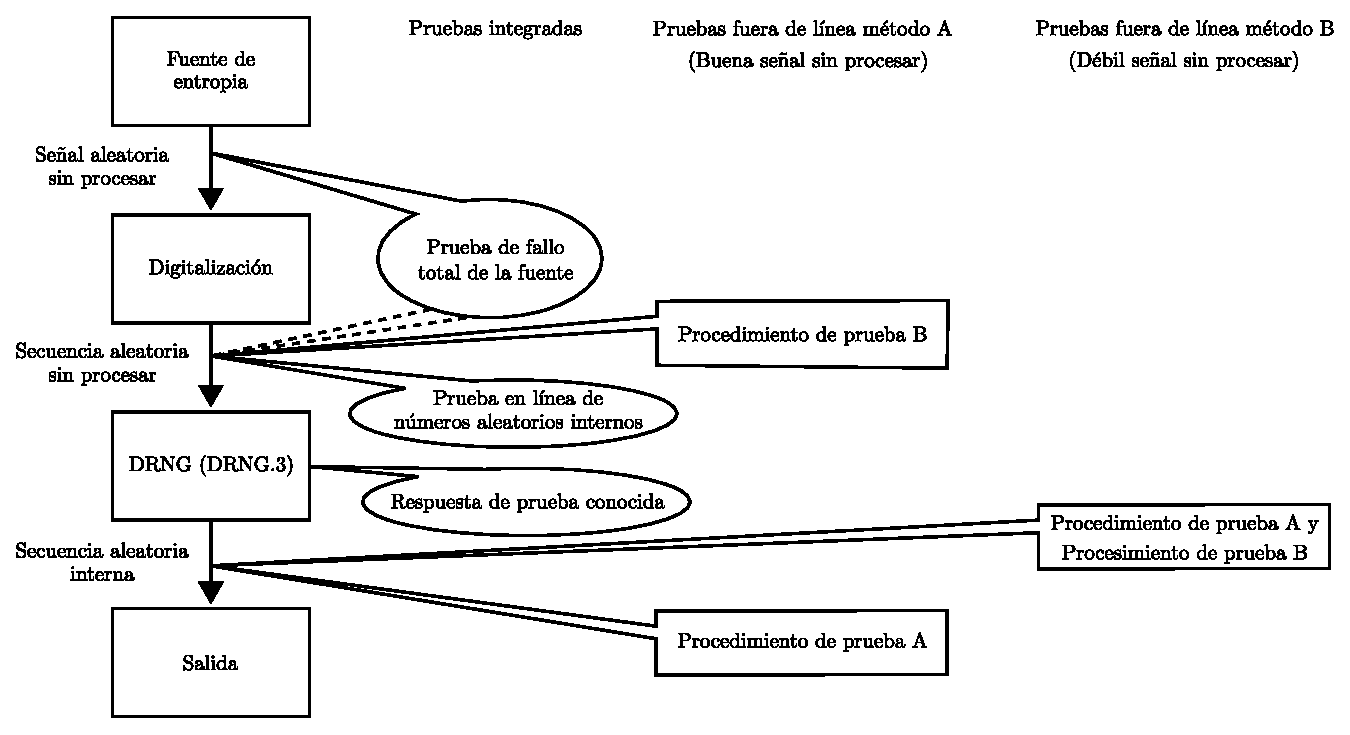
\includegraphics[width=0.9\textwidth]{E3_PTG3}
                    \label{fig:E3_PTG3}
                \end{figure}
            
                \paragraph{Requisitos de la fuente de aleatoriedad\\}
            
                La fuente de aleatoriedad del TRNG PTG.3 debe cumplir todos los requisitos de la clase PTG.2. La entropía de Shannon de la señal binaria sin procesar debe ser superior a 0.997 por bit, lo que debe estar garantizado por el modelo estocástico de la fuente.

                \paragraph{Pruebas integradas\\}
            
                Además de las pruebas de fallo total y en línea que se exigen también para el TRNG PTG.2, la clase PTG.3 requiere también la prueba de respuesta conocida (KAT) para el posprocesamiento. Esta prueba debe pasar con éxito cada vez que se inicie o reinicie el TRNG para verificar el correcto funcionamiento del algoritmo de posprocesamiento.
                
                \paragraph{Post-procesamiento\\}
            
                A diferencia de los requisitos de PTG.1 y PTG.2, la clase PTG.3 requiere el uso de un postprocesamiento criptográfico. Además, requiere el uso de un DRNG de la clase DRG.3, que proporciona secreto hacia delante y hacia atrás mejorado. Esto significa que el postprocesamiento para un TRNG de clase PTG.3 debe ser una función criptográfica.

            \subsubsection{Clase DRG.1 DRNG}

                La clase DRG.1 establece los requisitos para los RNG deterministas. Los RNG que cumplen con esta norma deben generar una secuencia de números aleatorios que sea indistinguible de la secuencia generada por un RNG ideal a través de simples pruebas estadísticas de caja negra. Además, los DRNG conformes con DRG.1 proporcionan secreto hacia adelante, lo que significa que la seguridad de la secuencia generada no se ve comprometida aunque un atacante tenga acceso a una porción previa de la secuencia. La Figura \ref{fig:E4_DRG1} muestra el diagrama de bloques de este generador.

                Los RNG que cumplen con la norma DRG.1 pueden ser útiles en aplicaciones que requieren datos frescos que difieran de las secuencias previamente generadas con una alta probabilidad. Por ejemplo, pueden ser utilizados para generar retos en protocolos criptográficos o vectores de inicialización en cifradores de bloques en modos especiales de funcionamiento, siempre que no sea necesario proteger la secuencia previa de números aleatorios. Los DRNG que cumplen con DRG.1 son también adecuados para pruebas de conocimiento cero. \cite{AIS2011}

                Para generar la semilla del DRNG se puede utilizar el PTRNG PTG.2 o PRG.3. Si el estado interno es al menos un 25 \% mayor en bits que los límites de entropía mínima, no es necesario una evaluación explícita de la entropía mínima. Esto se justifica por el hecho de que los PTRNG PTG.2 y PTG.3 generan números aleatorios de alta entropía.

                $\varphi$ es la función de transición de estado y $\psi$ es la función de salida

                \begin{figure}[hbtp]
                    \caption{Clase DRNG.1.}
                    \centering
                    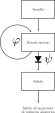
\includegraphics[width=0.2\textwidth]{E4_DRG1}
                    \label{fig:E4_DRG1}
                \end{figure}


        \subsection{Resumen de los requisitos del NIST 800-90B}
	
            El NIST 800-90B exige, al igual que el AIS-20/31, que la secuencia de salida del TRNG pase las pruebas de caja negra. Estas pruebas de caja negra se dividen en dos caminos:
            
            \begin{itemize}[noitemsep]
                \item IID track, se utiliza para datos independientes e idénticamente distribuidos o Independent and Identically Distributed en ingles (IID).
                \item Non-IID track, se utiliza para los datos que no superan la prueba de detección de IID.
            \end{itemize}

            Además de superar las pruebas de caja negra, el NIST 800-90B también impone requisitos a los bloques individuales del TRNG.
            
            \paragraph{Fuente de ruido\\}
            
                El NIST 800-90B tiene los siguientes requisitos sobre la fuente de ruido:
                
            \begin{itemize}[noitemsep]
                \item Su comportamiento debe estar descrito..
                \item Su salida debe ser estacionaria.
                \item Debe indicarse la entropía de salida esperada.
                \item Debe protegerse de la observación e influencia de los adversarios.
                \item La fuente de ruido debe tener un comportamiento aleatorio.
            \end{itemize}
            
            Aunque la norma exige la declaración de estacionariedad de la salida y de entropía esperada, no requiere ninguna prueba matemática de estas afirmaciones. Sólo es necesaria la descripción técnica de por qué se cree que la fuente de ruido tiene el comportamiento afirmado.
            
            \paragraph{Pruebas de salud\\}
            
            El NIST 800-90B exige tres tipos de pruebas de salud.
            
            \begin{itemize}[noitemsep]
                \item Las pruebas de puesta en marcha deben verificar si todos los componentes necesarios de la fuente de ruido funcionan correctamente. La fuente de ruido no debe emitir datos antes de que las pruebas de puesta en marcha se completen con éxito.
                \item Las pruebas continuas comprueban los defectos y fallos en el comportamiento de la fuente de ruido. Estas pruebas se realizan de forma continua en todas las muestras emitidas por la fuente de ruido. El NIST 800-90B exige que se utilicen dos pruebas continuas aprobadas. Además de las pruebas aprobadas, también se pueden utilizar pruebas definidas por el desarrollador. La norma permite a los desarrolladores no utilizar las pruebas aprobadas, pero en su lugar deben utilizarse otras pruebas continuas que pueden detectar el mismo tipo de defectos que las pruebas aprobadas.
                \item Las pruebas bajo demanda no se realizan hasta que se solicitan. Debe haber una forma de realizar pruebas bajo demanda en la fuente de ruido. Las muestras utilizadas para las pruebas bajo demanda no deben salir hasta que las pruebas se completen con éxito.
            \end{itemize}
            
            \paragraph{Acondicionamiento\\}
            
            El NIST 800-90B entiende por componente acondicionador una función determinista responsable de reducir el sesgo y/o aumentar la tasa de entropía de los bits de salida resultantes \cite{Turan2018}. El componente de acondicionamiento es completamente opcional, por lo que puede omitirse por completo.
            
            La entropía de salida del TRNG se estima después del componente de condicionamiento. El estándar proporciona una lista de algoritmos de condicionamiento comprobados, para los que los desarrolladores pueden reclamar una entropía completa, aunque esta reclamación tiene que ser validada. Estos algoritmos son funciones hash combinadas con cifrado de bloques, para ver la lista de componentes de acondicionamiento verificados ver \cite{Turan2018}.
            
            Se permite el uso de componentes de acondicionamiento no validados, pero estos componentes son penalizados en términos de estimación de entropía. Cuando se utiliza un componente condicionante no validado, la entropía en la salida se multiplica por una constante de 0.999, lo que le impide alcanzar la entropía total.

            Los parámetros recomendados para configurar las pruebas NIST se muestran en la Tabla \ref{tab:NIST_parametros}:

            \begin{table}[htbp]
                \caption{Parámetros recomendados para el conjunto de pruebas del NIST.}
                \begin{center}
                    \resizebox{0.8\linewidth}{!}{ 
                    \begin{NiceTabular}{|l|l|l|}
                        \CodeBefore
                        \rowcolor{lightgray}{1}
                        \Body
                        \hline
                        \textbf{Test}  & \textbf{Configuration item} & \textbf{Setting} \\
                        \hline
                        All tests   & Bits per sequence & 1000000  \\
                        \hline
                        All test   & Number of sequences (sample size) & 1073 \\
                        \hline
                        Frequency test within a block & Block length & 20000  \\
                        \hline
                        Non-overlapping template test  & Template length & 10  \\
                        \hline
                        Overlapping template & Block length & 10 \\
                        \hline
                        Mauler's Universal Statistical test  & Test block length L &  7 \\
                        \hline
                        Mauler's Universal Statistical test  & Initialization steps  &  1280 \\
                        \hline
                        Approximate entropy test & Block length &  8 \\
                        \hline
                        Linear complexity test  & Block length &  1000 \\
                        \hline
                        Serial test & Block length &  16 \\
                        \hline
                    \end{NiceTabular}
                    }
                \label{tab:NIST_parametros}
                \end{center}
            \end{table}
                    
		\subsection{Conclusiones de la certificación de seguridad TRNG}
		
            Hay dos normas principales relativas a los TRNG que están en vigor en la actualidad:
            
            \begin{itemize}[noitemsep]
                \item AIS-20/31 utilizado en muchos países europeos. \cite{AIS2011}
                \item NIST 800-90B utilizado en los Estados Unidos. \cite{Turan2018}
            \end{itemize}
        
            Las dos normas existentes en la actualidad exigen que el diseño de un TRNG esté bien documentado y su funcionamiento interno bien descrito, además de las pruebas estadísticas. También exigen que se realicen pruebas integradas, de modo que un TRNG se supervise continuamente durante su funcionamiento.
        
            Sin embargo, la norma AIS-20/31 profundiza en el problema de la descripción del TRNG y exige que se desarrolle también un modelo estocástico. Las pruebas integradas, según la AIS-20/31, también deben implementarse de acuerdo con el modelo estocástico. Este requisito no se aplica en la norma NIST 800-90B, que da más libertad en el diseño del TRNG, pero no en sus pruebas.

    \section{Fuentes de aleatoriedad en los dispositivos lógicos}

        \subsection{Jitter del reloj}

            Como se mencionó anteriormente, el jitter del reloj es una fuente confiable de aleatoriedad en dispositivos lógicos. El término ``jitter'' se refiere a la incertidumbre en la oscilación del reloj en el dominio del tiempo. En otras palabras, se trata de la variación a corto plazo de un evento con respecto a su posición ideal. Por lo general, se mide como la variación en el tiempo del cruce por cero (flanco ascendente o descendente) de la señal de reloj. Aunque esta definición proporciona una comprensión básica del concepto, cuantificar el jitter puede ser confuso debido a la variedad de técnicas de medición utilizadas en diferentes aplicaciones y a la falta de consenso entre los autores en la definición precisa del término.

            Se supone que una señal de reloj ideal en dispositivos lógicos digitales es una señal rectangular con un ciclo de trabajo del 50\% y un periodo estable. Pero debido a diversos ruidos que afectan a los dispositivos electrónicos, la señal de reloj nunca es absolutamente estable y sus bordes se mueven de su posición estable. En otras palabras, la fase de la señal de reloj fluctúa. Esta fluctuación puede verse como un jitter del reloj en el dominio del tiempo y como un ruido de fase en el dominio de la frecuencia. En los dispositivos lógicos, la fluctuación de reloj suele ser no deseada, pero inevitable. Dado que el jitter afecta negativamente a las comunicaciones de alta frecuencia y a los sistemas de alta velocidad, se ha estudiado y caracterizado en profundidad.

            En los sistemas analógicos, el jitter se caracteriza mejor en el dominio de la frecuencia. De este modo, los componentes de fase y amplitud pueden estudiarse y caracterizarse por separado. En cambio, en los sistemas digitales, las propiedades temporales del jitter son más importantes y, por tanto, el jitter se caracteriza en el dominio temporal.

            El jitter del reloj en un sistema digital es una desviación del flanco de reloj real con respecto a un flanco de reloj ideal. Una señal de reloj ideal se define mediante la ecuación (\ref{eq:señal_periodica}), donde $t(n)$ representa el tiempo del periodo $n$-ésimo de una señal de reloj y $T$ es el periodo de una señal de reloj.

            \begin{equation}
                t(n) = n \cdot T 
                \label{eq:señal_periodica}
            \end{equation}

            En la práctica, una señal de reloj real no alcanza siempre múltiplos enteros de su período ideal, sino que sus flancos fluctúan alrededor de este valor debido al jitter. Esta variación es causada por diversos fenómenos físicos, como el ruido térmico, el ruido de la fuente de alimentación y el ruido electromagnético ambiental, entre otros. La Figura \ref{fig:F9_jitter} muestra cómo se ve una señal de reloj afectada por el jitter.

            \begin{figure}[hbtp]
                \caption{Jitter del reloj.}
                \centering
                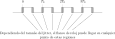
\includegraphics[width=0.8\textwidth]{F9_jitter}
                \label{fig:F9_jitter}
            \end{figure}
                
            La Figura \ref{fig:F10_fluctuaciones} muestra la causa principal del jitter en los circuitos digitales. Los circuitos digitales utilizan un nivel de referencia, generalmente ubicado en el centro del rango de voltaje de funcionamiento, para detectar los flancos de reloj. Es importante que este nivel de referencia sea lo más estable posible, pero en la práctica sufre fluctuaciones debido a diversos tipos de ruido. Cuando el nivel de referencia se desplaza, los flancos del reloj se detectan antes o después de lo previsto, lo que resulta en una variación temporal conocida como jitter de reloj.

            \begin{figure}[hbtp]
                \caption{Fluctuaciones del nivel de referencia originadas por ruidos analógicos que provocan jitter del reloj en los circuitos digitales. \cite{Petura2019}}
                \centering
                \includegraphics[width=0.8\textwidth]{F10_fluctuaciones}
                \label{fig:F10_fluctuaciones}
            \end{figure}
        
            A continuación se explican las diferentes medidas de jitter que observamos en circuitos digitales y las relaciones entre ellas.

            \subsection{Jitter de fase}

                El jitter de fase es una diferencia entre el tiempo del $n$-ésimo flanco de reloj real $t_{r}(n)$ y el tiempo (fase) del $n$-ésimo flanco de reloj ideal. La ecuación (\ref{eq:jitter_fase}) define esta relación.

                \begin{equation}
                    \delta_{\varphi}(n) = t_{r}(n) - n \cdot T_{\text{ref}}
                    \label{eq:jitter_fase}
                \end{equation}
                
                La Figura \ref{fig:F11_jitter_fase} ilustra este jitter para $n = 3.$. Para mayor claridad, sólo se muestra la fluctuación de fase de los flancos ascendentes, pero hay que tener en cuenta que la fluctuación de fase afecta a todos los flancos del reloj.

                \begin{figure}[hbtp]
                    \caption{Ilustración de la jitter de fase del segundo flanco ascendente de la señal de reloj. \cite{Petura2019}}
                    \centering
                    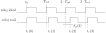
\includegraphics[width=0.8\textwidth]{F11_jitter_fase}
                    \label{fig:F11_jitter_fase}
                \end{figure}

                En la Figura \ref{fig:F11_jitter_fase} se muestra que el jitter de fase $\delta_{\varphi}(2)$ no solo se ve afectada por la desviación de fase de $t_{r}(2)$, sino que también contiene contribuciones a la desviación de $t_{r}(1)$. Esto se conoce como acumulación de fluctuación de fase y provoca que la fluctuación de fase observada aumente con $n$.

            \subsection{Jitter de periodo}

                El jitter de periodo es la diferencia entre un periodo de reloj real y el de uno ideal. Se define como se muestra en la ecuación (\ref{eq:jitter_periodo}), una diferencia de primer orden de la fluctuación de fase.

                \begin{eqnarray}
                    \delta_{T}(n) & = & [t_{r} (n) - t_{r} (n-1)] - T_{\text{ref}}\\
                                  & = & \delta_{\varphi}(n) - \delta_{\varphi}(n-1)
                    \label{eq:jitter_periodo}
                \end{eqnarray}

                La Figura \ref{fig:F12_jitter_periodo} muestra la fluctuación de los periodos. Podemos ver que los periodos reales cambian con el tiempo, a diferencia de los periodos ideales, que permanecen constantes.

                \begin{figure}[hbtp]
                    \caption{Ilustración de jitter de periodo de una señal de reloj real comparada con el reloj ideal.}
                    \centering
                    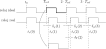
\includegraphics[width=0.8\textwidth]{F12_jitter_periodo}
                    \label{fig:F12_jitter_periodo}
                \end{figure}

            \subsection{Jitter de ciclo a ciclo}

                El jitter ciclo a ciclo es una diferencia de dos periodos de reloj reales consecutivos, tal y como se define en la ecuación (\ref{eq:jitter_ciclo}).
                
                \begin{eqnarray}
                    \delta_{c}(n) & = & T_{r} (n) - T_{r} (n-1)\\
                                  & = & [t_{r}(n) - t_{r}(n-1)] - [t_{r}(n-1) - t_{r}(n-2)] \\
                                  & = & \delta_{T}(n) - \delta_{T}(n-1)
                    \label{eq:jitter_ciclo}
                \end{eqnarray}

                Todas estas medidas de jitter están relacionadas entre sí, el jitter de periodo es la diferencia de primer orden del jitter de fase y el jitter ciclo a ciclo es la diferencia de primer orden del jitter de periodo. Por lo tanto, en general basta con medir sólo uno y calcular cualquier otro que pueda ser necesario. En la Figura \ref{fig:F13_jitter_ciclo} se muestra el jitter ciclo a ciclo.

                \begin{figure}[hbtp]
                    \caption{Ilustración de jitter de ciclo a ciclo.}
                    \centering
                    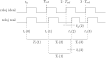
\includegraphics[width=0.8\textwidth]{F13_jitter_ciclo}
                    \label{fig:F13_jitter_ciclo}
                \end{figure}

            \subsection{Composición del jitter}

                El jitter del reloj suele tener dos componentes, ver la Figura \ref{fig:F14_jitter_componentes}, jitter aleatorio, causada por un fenómeno no determinista como el ruido térmico y jitter determinista, causada por algunos procesos deterministas.

                \begin{figure}[hbtp]
                    \caption{Composición del jitter del reloj.}
                    \centering
                    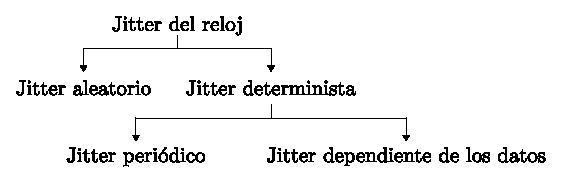
\includegraphics[width=0.6\textwidth]{F14_jitter_componentes}
                    \label{fig:F14_jitter_componentes}
                \end{figure}





        \subsection{Metaestabilidad}


    \section{Arquitectura de núcleos TRNGs en FPGA}

        Con base en los criterios del AIS-20/31, y los núcleos  que usan estructuras oscilantes como se clasifican en \cite{Petura2016}:
	
        \begin{itemize}
            \item Single-event ring oscillators
                \begin{itemize}
                    \item Elementary ring oscillator based TRNG 
                    \item Coherent sampling ring oscillator based TRNG 
                    \item Multi-ring oscillator based TRNG 
                \end{itemize}
            \item Multi-event ring oscillators with signal collisions
                \begin{itemize}
                    \item Transient effect ring oscillator based TRNG 
                \end{itemize}
            \item Multi-event ring oscillators without signal collisions
                \begin{itemize}
                    \item Self-timed ring based TRNG 
                \end{itemize}
            \item Phase-locked loops
                \begin{itemize}
                    \item PLL based TRNG 
                \end{itemize}
        \end{itemize}
	
		\subsection{Elementary ring oscillator based TRNG (ERO-TRNG)}
		
					
				\begin{figure}[hbtp]
					\caption{Arquitectura del núcleo ERO-TRNG.}
					\centering
					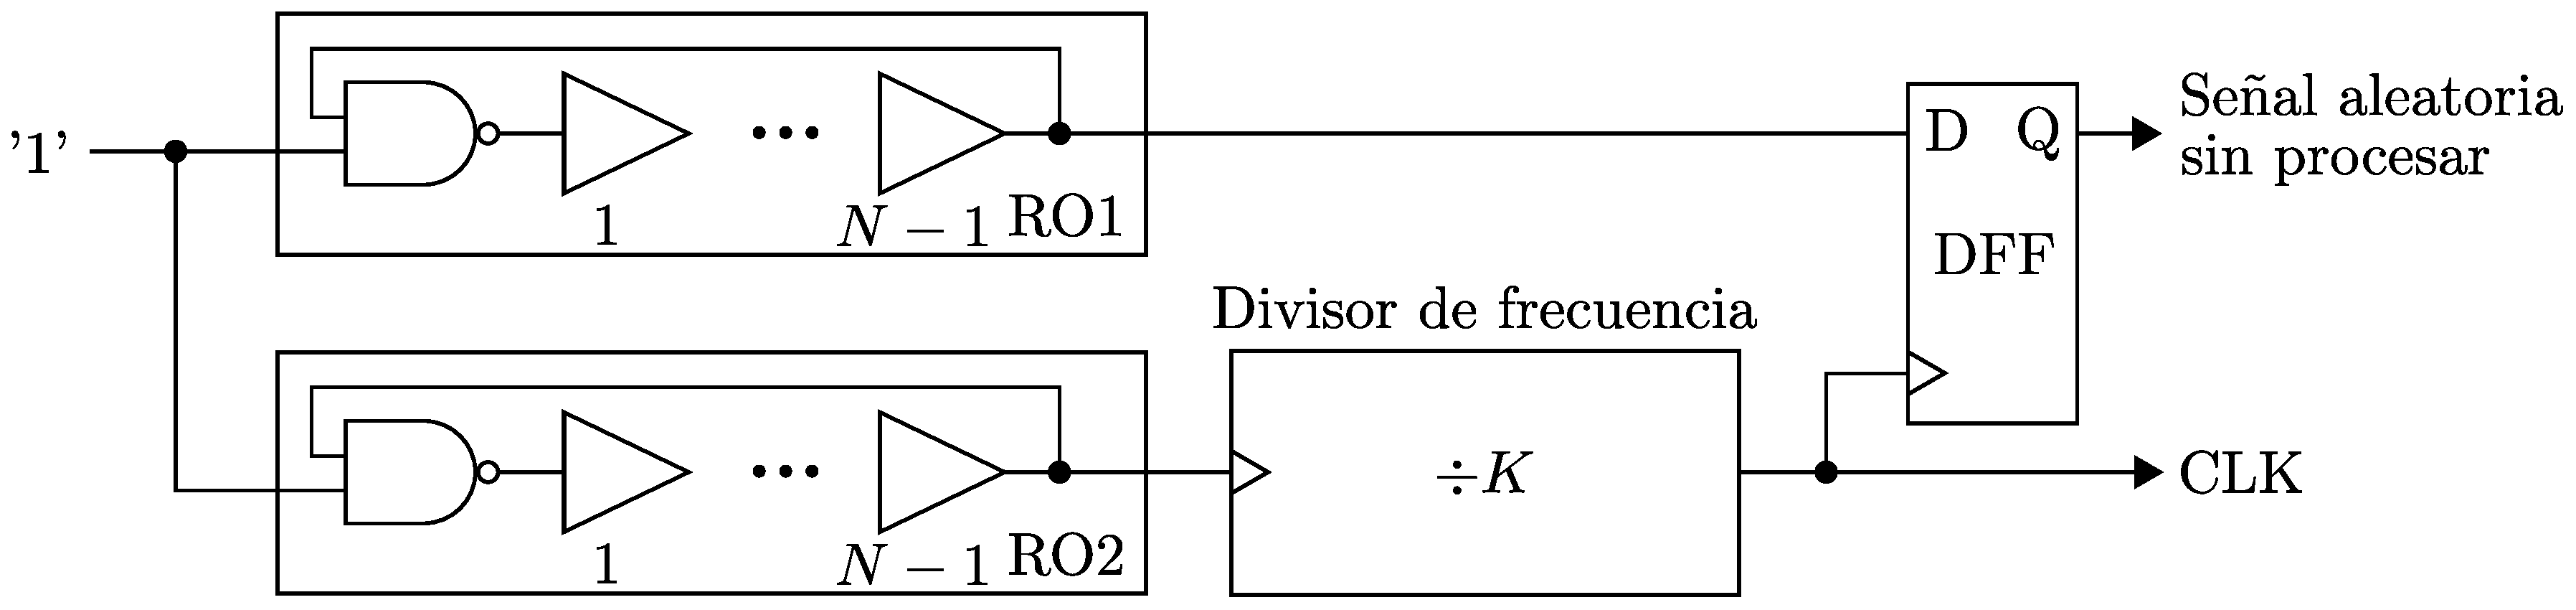
\includegraphics[width=0.8\linewidth]{A1_ERO_TRNG}
					\label{fig:A1_ERO_TRNG}
				\end{figure}
			
			
			
		\subsection{Coherent sampling ring oscillator based TRNG (COSO-TRNG)}
	
				
				\begin{figure}[hbtp]
					\caption{Arquitectura del núcleo COSO-TRNG.}
					\centering
					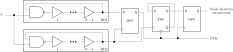
\includegraphics[width=0.8\linewidth]{A2_COSO_TRNG}
					\label{fig:A2_COSO_TRNG}
				\end{figure}
				
				
		\newpage		
		\subsection{Multi-ring oscillator based TRNG (MURO-TRNG)}
	
				
				\begin{figure}[hbtp]
					\caption{Arquitectura del núcleo MURO-TRNG.}
					\centering
					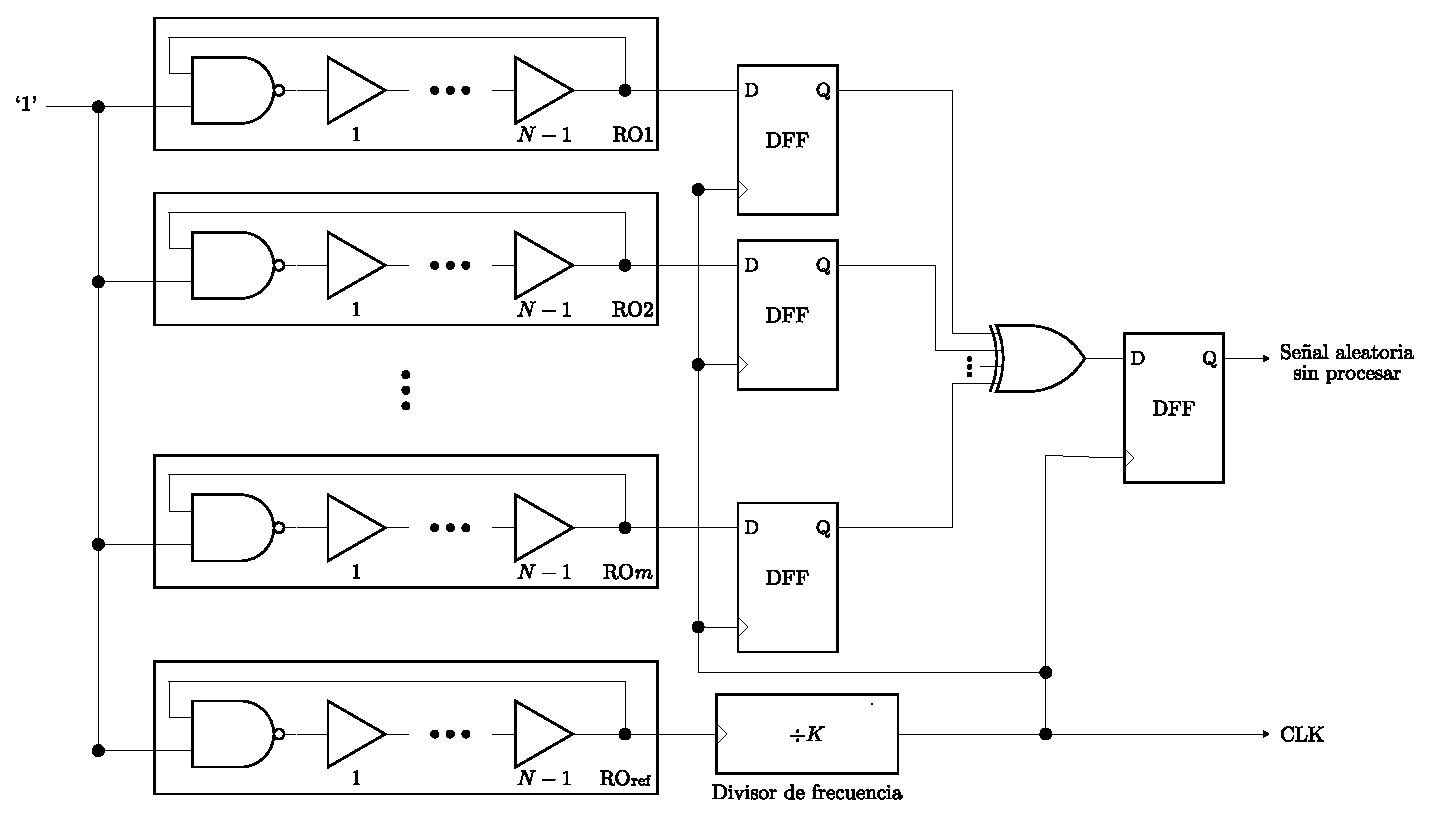
\includegraphics[width=0.8\linewidth]{A3_MURO_TRNG}
					\label{fig:A3_MURO_TRNG}
				\end{figure}
				
				
				
		\subsection{Transient effect ring oscillator based TRNG (TERO-TRNG)}
	
				
				\begin{figure}[hbtp]
					\caption{Arquitectura del núcleo TERO-TRNG.}
					\centering
					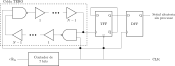
\includegraphics[width=0.8\linewidth]{A4_TERO_TRNG}
					\label{fig:A4_TERO_TRNG}
				\end{figure}
				
				
		\newpage	
		\subsection{Self-timed ring based TRNG (STR-TRNG)}
	
				
				\begin{figure}[hbtp]
					\caption{Arquitectura del núcleo STR-TRNG.}
					\centering
					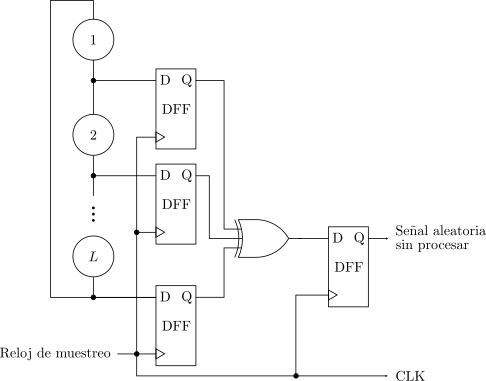
\includegraphics[width=0.8\linewidth]{A5_STR_TRNG}
					\label{fig:A5_STR_TRNG}
				\end{figure}
				
				
				
		\subsection{PLL based TRNG (PLL-TRNG)}
	
				
				\begin{figure}[hbtp]
					\caption{Arquitectura del núcleo PLL-TRNG.}
					\centering
					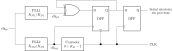
\includegraphics[width=0.8\linewidth]{A6_PLL_TRNG}
					\label{fig:A6_PLL_TRNG}
				\end{figure}
				
                \begin{table}[htbp]
                  \centering
                  \caption{Resumen de los resultados núcleos TRNGs}
                    \resizebox{0.8\linewidth}{!}{ 
                        \begin{tabular}{|c|c|c|c|c|c|c|c|c|}
                            \hline
                            \rowcolor{lightgray} TRNG Type & FPGA  & Area  & Power cons. & Bit Rate & Efficiency & Entropy & Entropy * Bit rate & Feasib. \\
                            \rowcolor{lightgray}       & device & (LUT/Reg) & [mW]  & [Mbits/s] & [bits/$\mu$Ws] & per bit &       & \& Repeat. \\
                            \hline
                            \multirow{3}[2]{*}{ERO} & Spartan 6 & 46/19 & 2.16  & 0.0042 & 1.94  & 0.999 & 0.004 & \multirow{3}[2]{*}{5} \\
                                  & Cyclone V & 34/20 & 3.24  & 0.0027 & 0.83  & 0.990 & 0.003 &  \\
                                  & SmartFusion 2 & 45/19 & 4     & 0.014 & 3.5   & 0.980 & 0.013 &  \\
                            \hline
                            \multirow{3}[2]{*}{COSO} & Spartan 6 & 18/3  & 1.22  & 0.54  & 442.6 & 0.999 & 0.539 & \multirow{3}[2]{*}{1} \\
                                  & Cyclone V & 13/3  & 0.9   & 1.44  & 1600  & 0.999 & 1.438 &  \\
                                  & SmartFusion 2 & 23/3  & 1.94  & 0.328 & 169   & 0.999 & 0.327 &  \\
                            \hline
                            \multirow{3}[2]{*}{MURO} & Spartan 6 & 521/131 & 54.72 & 2.57  & 46.9  & 0.999 & 2.567 & \multirow{3}[2]{*}{4} \\
                                  & Cyclone V & 525/130 & 34.93 & 2.2   & 62.9  & 0.999 & 2.197 &  \\
                                  & SmartFusion 2 & 545/130 & 66.41 & 3.62  & 54.5  & 0.999 & 3.616 &  \\
                            \hline
                            \multirow{3}[2]{*}{PLL} & Spartan 6 & 34/14 & 10.6  & 0.44  & 41.5  & 0.981 & 0.431 & \multirow{3}[2]{*}{3} \\
                                  & Cyclone V & 24/14 & 23    & 0.6   & 43.4  & 0.986 & 0.592 &  \\
                                  & SmartFusion 2 & 30/15 & 19.7  & 0.37  & 18.7  & 0.921 & 0.340 &  \\
                            \hline
                            \multirow{3}[2]{*}{TERO} & Spartan 6 & 39/12 & 3.312 & 0.625 & 188.7 & 0.999 & 0.624 & \multirow{3}[2]{*}{1} \\
                                  & Cyclone V & 46/12 & 9.36  & 1     & 106.8 & 0.987 & 0.985 &  \\
                                  & SmartFusion 2 & 46/12 & 1.23  & 1     & 813   & 0.999 & 0.999 &  \\
                            \hline
                            \multirow{3}[2]{*}{STR} & Spartan 6 & 346/256 & 65.9  & 154   & 2343.2 & 0.998 & 154.121 & \multirow{3}[2]{*}{2} \\
                                  & Cyclone V & 352/256 & 49.4  & 245   & 4959.1 & 0.999 & 244.755 &  \\
                                  & SmartFusion 2 & 350/256 & 82.52 & 188   & 2286.7 & 0.999 & 188.522 &  \\
                            \hline
                        \end{tabular}%
                    }
                  \label{tab:resumen_de_trng_cores}
                \end{table}%


	\chapter{Implementación}

	\section{Mapa caótico}
    
        En el artículo \cite{Sprott1993} y \cite{Fraga2021}
        \begin{equation}
            \begin{array}{ccl}
                x_{n+1} & = &  a_{1} + a_{2}x_{n} + a_{3}x_{n}^{2} + a_{4}x_{n}y_{n} + a_{5}y_{n} + a_{6}y_{n}^{2}\\
                y_{n+1} & = &  a_{7} + a_{8}x_{n} + a_{9}x_{n}^{2} + a_{10}x_{n}y_{n} + a_{11}y_{n} + a_{12}y_{n}^{2}
            \end{array}
        \end{equation}
        
        donde los parámetros $\{a_{1}, a_{2}, \ldots a_{12}\}$ pueden tomar diferentes valores, sin embargo para este trabajo se usaron los siguientes:


        \begin{equation}
            \begin{array}{ccl}
                x_{n+1} & = &  a_{1} + ( a_{2} + a_{3}x_{n} )x_{n} + a_{4}x_{n}y_{n} + ( a_{5} + a_{6}y_{n} )y_{n} \\
                y_{n+1} & = &  a_{7} + ( a_{8} + a_{9}x_{n} )x_{n} + a_{10}x_{n}y_{n} + ( a_{11} + a_{12}y_{n})y_{n}
            \end{array}
        \end{equation}

        \begin{equation}
             \begin{array}{lcl}
                M_{1} & = & \{ -0.6, -0.1, 1.1, 0.2, -0.8, 0.6, -0.7, 0.7, 0.7, 0.3, 0.6, 0.9 \}\\
                M_{2} & = & \{ -1.0, 0.9, 0.4, -0.2, -0.6, -0.5, 0.4, 0.7, 0.3, -0.5, 0.7, -0.8 \}\\
                M_{3} & = &  \{0.8, 1.0, -1.2, -1.0, 1.1, -0.9, 0.4, -0.4, -0.6, -0.2, -0.5, -0.7 \}\\
                M_{4} & = & \{-0.6, -0.4, -0.4, -0.8, 0.7, 0.3, -0.4, 0.4, 0.5, 0.5, 0.8, -0.1 \}
            \end{array}
        \end{equation}

        \begin{equation}
            \begin{array}{lcl}
                s_{n+1} = \{ x_{n+1} \text{ mod } 256, y_{n+1} \text{ mod } 256 \}
            \end{array}
        \end{equation}

        \begin{table}[htbp]
            \centering
            \caption{Exponentes de Lyapunov y dimensión fractal (tomados de \cite{Sprott1993}) de los mapas 2D usados.}
            \begin{tabular}{|l|l|l|}
                \hline
                \rowcolor[rgb]{ .682,  .667,  .667}Mapa  & Exponentes de Lyapunov & Dimensión fractal \\
                \hline
                1     & 0.12                   & 1.77   \\
                \hline
                2     & 0.14                   & 1.79   \\
                \hline
                3     & 0.15                   & 1.69   \\
                \hline
                4     & 0.13                   & 1.50   \\
                \hline
            \end{tabular}
        \end{table}

        \begin{table}[htbp]
            \centering
            \caption{Número de bits usados en la implementación de cada uno de los mapas con aritmética de punto fijo.}
            \begin{tabular}{|l|l|l|}
                \hline
                \rowcolor[rgb]{ .682,  .667,  .667}Mapa  & Bits parte entera & Bits parte fraccionaria \\
                \hline
                1     & 3                   & 60   \\
                \hline
                2     & 4                   & 59   \\
                \hline
                3     & 4                   & 59   \\
                \hline
                3     & 3                   & 60   \\
                \hline
            \end{tabular}
        \end{table}

        \begin{table}[htbp]
            \centering
            \caption{Rangos usados para la condición inicial para cada uno de los mapas.}
            \begin{tabular}{|l|l|}
                \hline
                \rowcolor[rgb]{ .682,  .667,  .667}Mapa  & Rango de valores para $x_{0}$ y $y_{0}$ \\
                \hline
                $M_{1}$  & $x_{0} \in [-0.5, \phantom{-} 0.5]$, $y_{0} \in [-0.5, \phantom{-}0.5]$ \\
                \hline
                $M_{2}$  & $x_{0} \in [-1.0, \phantom{-} 0.0]$, $y_{0} \in [\phantom{-}0.0, \phantom{-}1.0]$ \\
                \hline
                $M_{3}$  & $x_{0} \in [\phantom{-}0.0, \phantom{-} 1.0]$, $y_{0} \in [-0.6, \phantom{-}0.4]$ \\
                \hline
                $M_{4}$  & $x_{0} \in [-1.5, -0.5]$, $y_{0} \in [-0.5, \phantom{-}0.5]$ \\
                \hline
            \end{tabular}
        \end{table}

        \begin{figure}[hbtp]
            \caption{Diagrama de bloques del mapa caótico.}
            \centering
            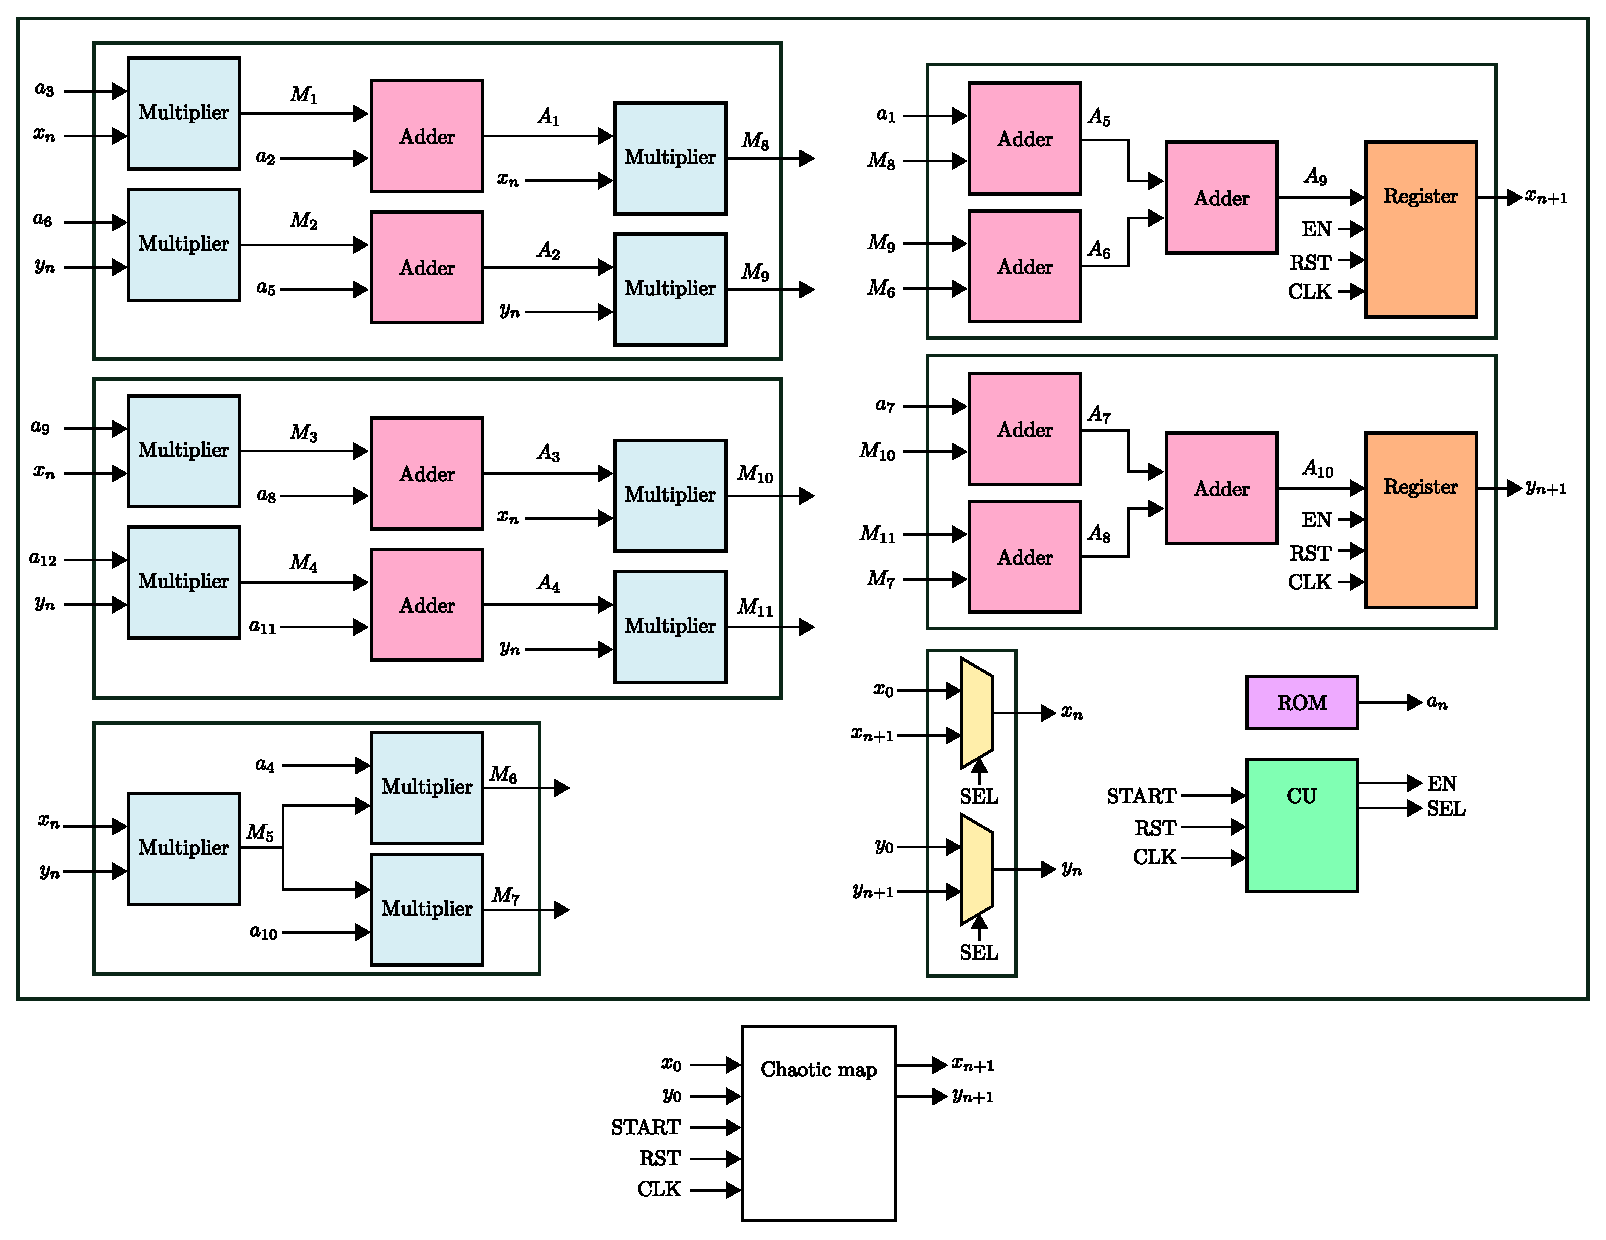
\includegraphics[width=0.9\linewidth]{B1_architecture}
            \label{fig:B1_architecture}
        \end{figure}

        \begin{figure}[hbtp]
            \caption{Máquina de estados de mapa caótico.}
            \centering
            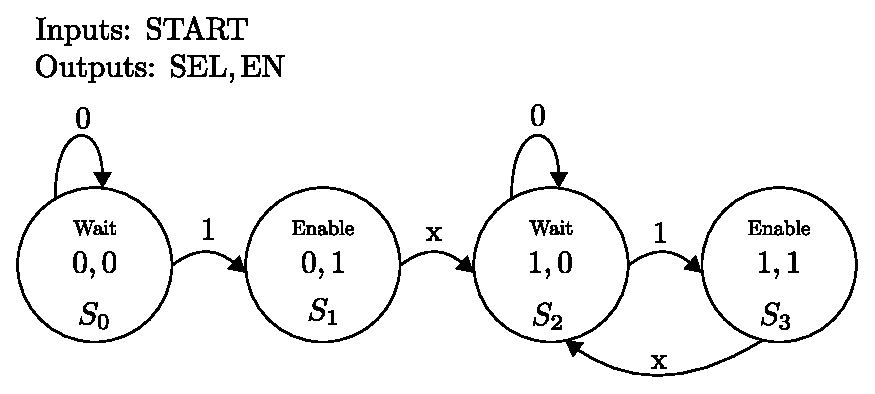
\includegraphics[width=0.6\linewidth]{B2_fsm_cm}
            \label{fig:B2_fsm_cm}
        \end{figure}

        \begin{figure}[hbtp]
            \caption{Simulación del mapa caótico en punto flotante.}
            \centering
            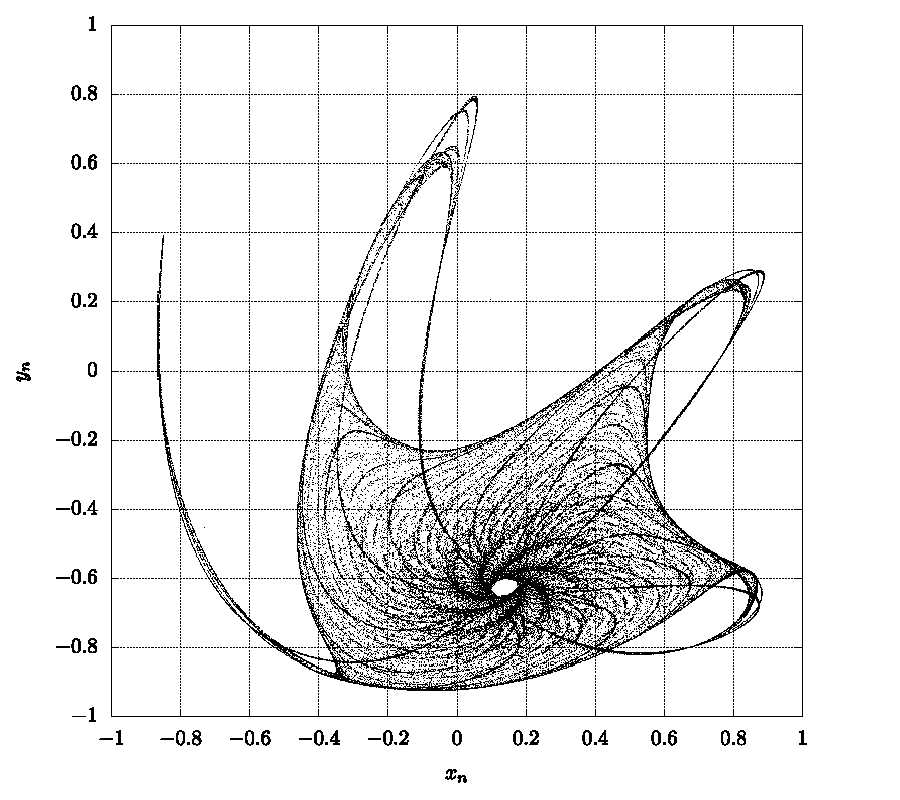
\includegraphics[width=0.8\linewidth]{B0_chaotic_map}
            \label{fig:B0_chaotic_map}
        \end{figure}

    \section{Single Constant Multiplier (SCM)}


    \section{Comunicación RS232}

        \begin{figure}[hbtp]
            \caption{Diagrama de bloques de transmisión RS232.}
            \centering
            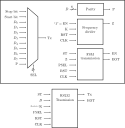
\includegraphics[width=0.6\linewidth]{C1_architecture_rs232}
            \label{fig:C1_architecture_rs232}
        \end{figure}

        \begin{figure}[hbtp]
            \caption{Máquina de estados para la transmisión RS232.}
            \centering
            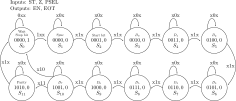
\includegraphics[width=0.8\linewidth]{C0_fsm_rs232}
            \label{fig:C0_fsm_rs232}
        \end{figure}	

    \section{Diseño de TRNG}

        \begin{figure}[hbtp]
            \caption{Diagrama de bloques de TRNG.}
            \centering
            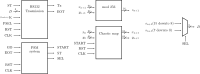
\includegraphics[width=0.9\linewidth]{D0_system}
            \label{fig:D0_system}
        \end{figure}

        \begin{figure}[hbtp]
            \caption{Máquina de estados de TRNG.}
            \centering
            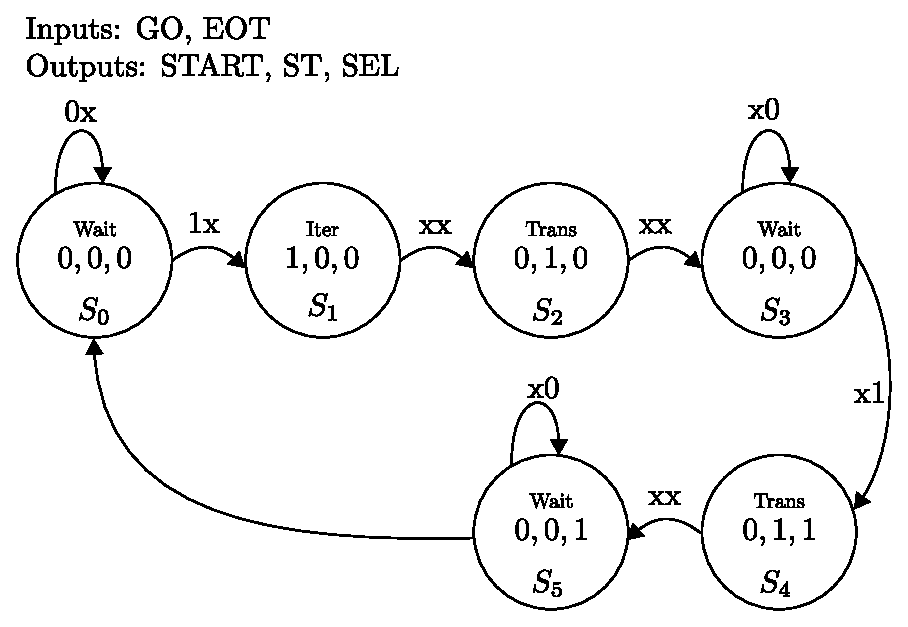
\includegraphics[width=0.7\linewidth]{D1_fsm_system}
            \label{fig:D1_fsm_system}
        \end{figure}

	\begin{comment}

	
\begin{table}[htbp]
  \centering
  \caption{Resumen de los resultados de implementación de las TRNGs}
\resizebox{0.5\linewidth}{!}{ 
    \begin{tabular}{lll}
   & Test name                 & Prop. \\
   \hline
1  & Frequency                 & 0.99  \\
2  & Block frequency           & 0.99  \\
3  & Runs                      & 1.00     \\
4  & Longest run               & 1.0     \\
5  & Rank                      & 0.98  \\
6  & DFT                       & 0.99  \\
7  & Non-overlapping templates & 1.00     \\
8  & Overlapping templates     & 0.99  \\
9  & Universal                 & 0.99  \\
10 & Linear complexity         & 0.99  \\
11 & Serial                    & 0.99  \\
12 & Approximate Entropy       & 0.99  \\
13 & Cumulative Sums           & 0.99  \\
14 & Random excursions         & 0.99  \\
15 & Random excursions variant & 1.00    
    \end{tabular}
}
  \label{tab:asdasd}
\end{table}


\newpage
	




	\end{comment}


	\chapter{Resultados experimentales}




	\chapter{Conclusiones}


	\chapter{Conclusiones}

	Comprobación de glosarios

\Gls{FPGA} 

\Gls{RNG} 

\Gls{TRNG}

\Gls{TERO}

\Gls{ERO-TRNG}

\Gls{COSO-TRNG}

\Gls{MURO-TRNG}

\Gls{TERO-TRNG}

\Gls{PLL-TRNG}

\Gls{STR-TRNG}


\appendix
	\chapter{Códigos}

%\lstinputlisting[style = MATLAB, caption =  Nombre de abajo, label = cod:nombre1]{codigos/matlab/test_code.m}

	\section{Códigos en C}
\lstinputlisting[style = C, caption =  Comprobar el número de bytes de los tipos de dato del sistema., label = cod:A1]{codigos/c_codes/A1_check_sys_bytes.c}

\newpage
\lstinputlisting[style = C, caption =  Simulación de mapa caótico en punto flotante., label = cod:A2]{codigos/c_codes/A2_chaotic_map_float.c}

\newpage
\lstinputlisting[style = C, caption =  Simulación de mapa caótico en punto fijo., label = cod:A3]{codigos/c_codes/A3_chaotic_map_fixed.c}

\newpage
\lstinputlisting[style = C, caption = Generador de memoria ROM de condiciones iniciales., label = cod:A4]{codigos/c_codes/A4_rom_gen_chaotic_map.c}

\newpage
\lstinputlisting[style = C, caption =  Convertidor de punto flotante a punto fijo., label = cod:A5]{codigos/c_codes/A5_fixed_point_converter.c}

\newpage
\lstinputlisting[style = C, caption = Simulación de mapa caótico en punto fijo y operación mod 256., label = cod:A6]{codigos/c_codes/A6_chaotic_map_mod.c}

\newpage
\lstinputlisting[style = C, caption = Simulación de mapa caótico en punto fijo y operación mod 256 salida binaria., label = cod:A7]{codigos/c_codes/A7_chaotic_map_mod_bin.c}

    \section{Códigos en VHDL de mapa caótico}

\lstinputlisting[style = VHDL, caption = Multiplexor para control de condición inicial y retroalimentación., label = cod:mux_ic]{codigos/vhdl_codes/chaotic_map/mux_ic.vhd}

\lstinputlisting[style = VHDL, caption = Sumador genérico compatible con punto fijo., label = cod:adder]{codigos/vhdl_codes/chaotic_map/adder.vhd}

\newpage
\lstinputlisting[style = VHDL, caption = ROM para almacenar parámetros en punto fijo del mapa caótico., label = cod:rom_cm]{codigos/vhdl_codes/chaotic_map/rom_cm.vhd}

\lstinputlisting[style = VHDL, caption = Multiplicador en punto fijo con truncamiento., label = cod:mult]{codigos/vhdl_codes/chaotic_map/mult.vhd}

\lstinputlisting[style = VHDL, caption = Flip-Flop con habilitación., label = cod:ff_hab]{codigos/vhdl_codes/chaotic_map/ff_hab.vhd}

% \newpage
\lstinputlisting[style = VHDL, caption = Máquina de estados para control de las iteraciones del mapa caótico., label = cod:fsm_cm]{codigos/vhdl_codes/chaotic_map/fsm_cm.vhd}

% \newpage
\lstinputlisting[style = VHDL, caption = Descripción completa del mapa caótico., label = cod:chaotic_map]{codigos/vhdl_codes/chaotic_map/chaotic_map.vhd}


% \newpage
% 	\section{Códigos en VHDL de comunicación RS232}
% \lstinputlisting[style = VHDL, caption = Divisor de frecuencia., label = cod:freq_div]{codigos/vhdl_codes/rs232/freq_div.vhd}

% \newpage
% \lstinputlisting[style = VHDL, caption = Detector de paridad tipo par., label = cod:parity]{codigos/vhdl_codes/rs232/parity.vhd}

% \lstinputlisting[style = VHDL, caption = Multiplexor para la selección de bits de la comunicación., label = cod:mux_trans]{codigos/vhdl_codes/rs232/mux_trans.vhd}

% \newpage
% \lstinputlisting[style = VHDL, caption = Transmisión del protocolo RS232., label = cod:transmission]{codigos/vhdl_codes/rs232/transmission.vhd}

% \lstinputlisting[style = VHDL, caption = Testbench de comunicación RS232., label = cod:tb_trans]{codigos/vhdl_codes/rs232/tb_trans.vhd}

% \newpage
% \lstinputlisting[style = VHDL, caption = Máquina de estados para el control de la transmisión., label = cod:fsm_trans]{codigos/vhdl_codes/rs232/fsm_trans.vhd}

% 	\section{Códigos en VHDL de ERO}


% \newpage
% 	\section{Códigos en VHDL de arquitectura TRNG}
% \lstinputlisting[style = VHDL, caption = Multiplexor para conexión con la comunicación RS232., label = cod:mux_system_mod]{codigos/vhdl_codes/trng/mux_system_mod.vhd}

% \lstinputlisting[style = VHDL, caption = Operación mod 256., label = cod:mod_256]{codigos/vhdl_codes/trng/mod_256.vhd}

% \newpage
% \lstinputlisting[style = VHDL, caption = Máquina de estados de sistema TRNG., label = cod:fsm_system_mod]{codigos/vhdl_codes/trng/fsm_system_mod.vhd}

% \newpage
% \lstinputlisting[style = VHDL, caption = Descripción de arquitectura TRNG., label = cod:system_mod]{codigos/vhdl_codes/trng/system_mod.vhd}


\backmatter

%\nocite{*}
\bibliographystyle{ieeetr}
\bibliography{bibliografia}

\end{document}
